\documentclass[a4paper, 11pt]{report}

% --- 提出モード設定 (1:提出用/白背景, 0:デバッグ用/黒背景) ---
\newcommand{\submissionmode}{1} 

% --- 高圧縮-  PDFの圧縮率を最大にする
% \pdfvariable minorversion=5
% \pdfvariable compresslevel=9
% \pdfvariable objcompresslevel=3

% --- Load settings ---
%===============================================================================
% This file is based on the following source:
%
% ファイル名: master_ja_sample.tex
% 作成者:サイトウ リョウタ(2024年度山上研究室 修士修了)
% 作成日:2025年2月19日
% https://github.com/ryota-saito-coastal/LaTeXsample_for_Kyoto-u_civileng_mthesis
%===============================================================================

% --- 基本パッケージ ---
\usepackage{luatexja}
\usepackage{luatexja-fontspec}
\usepackage[haranoaji]{luatexja-preset}

\usepackage{amsmath,amssymb,amsthm}% 数式関連のパッケージ
\usepackage{empheq} % 数式に括弧
\usepackage{mathtools}
\mathtoolsset{showonlyrefs=true}
\usepackage[unicode=true,hypertexnames=false,setpagesize=false,colorlinks=true,urlcolor=blue,linkcolor=blue,citecolor=blue]{hyperref}
\usepackage{cleveref}
\crefname{equation}{式}{式}% {環境名}{単数形}{複数形} \crefで引くときの表示
\crefname{figure}{図}{図}% {環境名}{単数形}{複数形} \crefで引くときの表示
\crefname{table}{表}{表}% {環境名}{単数形}{複数形} \crefで引くときの表示
\crefname{algorithm}{Algorithm}{Algorithm}

\crefname{section}{第}{第}
\creflabelformat{section}{#2#1節#3}
\crefname{subsection}{第}{第}
\creflabelformat{subsection}{#2#1小節#3}

\theoremstyle{definition}% 日本語用.定理とか斜体にならないようにする
\newtheorem{theorem}{定理}
\crefname{theorem}{定理}{定理}
\newtheorem{lemma}{補題}
\crefname{lemma}{補題}{補題}
\newtheorem{corollary}{系}
\crefname{corollary}{系}{系}
\newtheorem*{proof*}{証明}
\crefname{proof*}{証明}{証明}
\newtheorem{assumption}{仮定}
\crefname{assumption}{仮定}{仮定}
\newtheorem{definition}{定義}
\crefname{definition}{定義}{定義}
\newtheorem{remark}{注意}
\crefname{remark}{注意}{注意}
\newtheorem{proposition}{命題}
\crefname{proposition}{命題}{命題}


\newcommand{\crefpairconjunction}{と}
\newcommand{\crefrangeconjunction}{から}
\newcommand{\crefmiddleconjunction}{,}
\newcommand{\creflastconjunction}{,および} 
\usepackage{mathtools}

\usepackage{physics}
\usepackage[ppl]{mathcomp}
\usepackage{bm}
\usepackage{siunitx}
\usepackage{graphicx}
\usepackage{subcaption}
\usepackage{float}       % [H] オプション用
\usepackage{booktabs}    % 表の罫線(topruleなど)
\usepackage{xltabular}
\usepackage{makecell}
\usepackage{xcolor}
\usepackage{ifthen}
\usepackage{geometry}
\usepackage{setspace}
\usepackage{titlesec}
\usepackage{fancyhdr}
\usepackage{tocloft}
\usepackage{indentfirst} % 章の最初の段落も字下げ
\usepackage{bookmark}
\usepackage{caption}
\usepackage{enumitem}
\usepackage{url}
\usepackage{tabularx}   % For adjustable column widths
\usepackage{ragged2e}   % For better text alignment

% algorithm2e: アルゴリズムを書くためのパッケージ
\usepackage[ruled,vlined]{algorithm2e}
% ruled: 罫線を表示
% vlined: ブロックの縦線を表示
\SetKwComment{Comment}{// }{} 

\usepackage[colorinlistoftodos]{todonotes} % TODO用。Writing以外の思いついたEditingタスクを瞬時に外部化し、ワーキングメモリを解放
% --- 参考文献設定 (Biber + BibLaTeX) ---
% 従来の \usepackage{cite} や thebibliography環境 の代わり
\usepackage[backend=biber, style=phys, sorting=none]{biblatex} % style=numeric → style=physics

% --- 参考文献リストのスタイル設定 ---
% 1. 参考文献リスト内の行間を「1.0 (シングル)」に強制変更 ※ 全体の \linespread{2.5} をここだけ無効化
\AtBeginBibliography{\setstretch{1.0}} 
% 2. 項目ごとのフォントサイズを少し小さくする(任意) ※ 必要なければ \small を削除してください
% \renewcommand*{\bibfont}{\small}
% 3. 文献アイテム同士の間隔を詰める
\setlength{\bibitemsep}{2.5pt} % 項目間の余白 (0ptでも可)
\setlength{\bibparsep}{1.0pt}  % 項目内の段落間余白

% % 引用番号のスタイルを [1] から 1) に変更
% \DeclareFieldFormat{labelnumberwidth}{#1)}

% % 文中の引用 \cite{} を上付き文字にする設定
% \DeclareCiteCommand{\cite}[\mkbibsuperscript]
%   {\usebibmacro{cite:init}%
%    \usebibmacro{prenote}}
%   {\usebibmacro{citeindex}%
%    \printfield{labelnumber}\printtext{)}} % 閉じ括弧 ) を追加
%   {\multicitedelim}
%   {\usebibmacro{postnote}}

% 複数の引用をカンマ区切りにする
\renewcommand*{\multicitedelim}{\textsuperscript{,}}

% --- フォント設定 (LuaLaTeX用) ---
% 英数字フォント
\setmainfont{Times New Roman}[RawFeature={+palt, +kern}, LetterSpace=2.0]
\setsansfont{Arial}[RawFeature={+palt, +kern}, LetterSpace=1.5]
\setmonofont{Courier New}[RawFeature={+palt, +kern}, LetterSpace=1.0]

% 日本語フォント(必要に応じて有効化してください)
% \setmainjfont{MS Mincho}[RawFeature={+palt, +kern}, LetterSpace=12.5]
% \setsansjfont{MS Gothic}[RawFeature={+palt, +kern}, LetterSpace=10.0]
% \renewcommand{\bfseries}{\gtfamily}

% --- ページレイアウト ---
\geometry{left=20mm, right=20mm, top=25mm, bottom=25mm}
\setstretch{1.2} % 1.2倍行間

% --- キャプション等の日本語化 ---
\renewcommand{\figurename}{\normalfont\gtfamily 図}
\renewcommand{\tablename}{\normalfont\gtfamily 表}
\renewcommand{\contentsname}{\normalfont\gtfamily 目次}
\renewcommand{\thefigure}{\thechapter-\arabic{figure}}
\renewcommand{\thetable}{\thechapter-\arabic{table}}

% --- 見出しデザイン (titlesec) ---
\titleformat{\chapter}
    {\normalfont\fontsize{20pt}{24pt}\gtfamily}
    {第\hspace{2pt}\thechapter 章}
    {20pt}
    {\fontsize{20pt}{10pt}\selectfont}

\titleformat{\section}{\normalfont\fontsize{12pt}{12pt}\gtfamily}{\thesection}{1em}{}
\titleformat{\subsection}{\normalfont\fontsize{12pt}{12pt}\gtfamily}{\thesubsection}{1em}{}

% --- 目次設定 (tocloft) ---
\renewcommand{\cftchappresnum}{第}
\renewcommand{\cftchapaftersnum}{章\hspace{0.5em}}
\setlength{\cftchapnumwidth}{4.0em}

% --- ヘッダー・フッター ---
\pagestyle{fancy}
\fancyhf{}
\fancyfoot[C]{\thepage}
\renewcommand{\headrulewidth}{0pt}

% --- 便利コマンド ---
\newcommand{\HRule}[1]{\rule{1\linewidth}{#1}}
\newcommand{\percent}{\%}
\newcommand{\figureref}[1]{図\ref{#1}}
\newcommand{\tableref}[1]{表\ref{#1}}



% --- TODO用コマンド ---
% 要修正:赤(論理の飛躍、間違いなど)
\newcommand{\fix}[1]{\todo[inline, color=red!40, bordercolor=red, size=\small]{#1}}
% 要確認・出典:青(事実確認、引用もと探し)
\newcommand{\checkref}[1]{\todo[inline, color=blue!30, bordercolor=blue, size=\small]{#1}}
% 表現・推敲:緑(英語の言い回し、日本語のニュアンス)
\newcommand{\rewrite}[1]{\todo[inline, color=green!40, bordercolor=green, size=\small]{#1}}
% 自分へのメモ:黄色(デフォルト)
\newcommand{\note}[1]{\todo[inline, size=\small]{#1}}
% 小林先生のコメント
\newcommand{\kobayashi}[1]{\todo[inline, color=gray!40, bordercolor=gray, size=\small]{#1}}


% --- 図
\newcommand{\IncludeThreeImages}[9][3cm]{% [デフォルト高さは3cm]
  \begin{figure}[htbp]
    \centering
    % --- 1枚目 ---
    \begin{subfigure}[t]{0.32\textwidth}
      \centering
      \includegraphics[height=#1, keepaspectratio]{#2}
      \caption{#3} % 自動で(a)が入ります
    \end{subfigure}
    \hfill
    % --- 2枚目 ---
    \begin{subfigure}[t]{0.32\textwidth}
      \centering
      \includegraphics[height=#1, keepaspectratio]{#4}
      \caption{#5}
    \end{subfigure}
    \hfill
    % --- 3枚目 ---
    \begin{subfigure}[t]{0.32\textwidth}
      \centering
      \includegraphics[height=#1, keepaspectratio]{#6}
      \caption{#7}
    \end{subfigure}
    % --- 全体設定 ---
    \caption{#8}
    \label{#9}
  \end{figure}
}
% \IncludeThreeImages[4cm]
%   {img1.jpg}{キャプション1}
%   {img2.jpg}{キャプション2}
%   {img3.jpg}{キャプション3}
%   {全体キャプション}
%   {fig:test}
\newcommand{\IncludeTwoImages}[7][4cm]{% [デフォルト高さは3cm]
  \begin{figure}[htbp]
    \centering
    % --- 1枚目 ---
    \begin{subfigure}[t]{0.45\textwidth}
      \centering
      \includegraphics[height=#1, keepaspectratio]{#2}
      \caption{#3} % 自動で(a)が入ります
    \end{subfigure}
    \hspace{0.5cm}
    % --- 2枚目 ---
    \begin{subfigure}[t]{0.45\textwidth}
      \centering
      \includegraphics[height=#1, keepaspectratio]{#4}
      \caption{#5}
    \end{subfigure}
    % --- 全体設定 ---
    \caption{#6}
    \label{#7}
  \end{figure}
}


% --- デバッグモード設定 (目に優しい黒背景) ---
% \submissionmode は main.tex で定義する
\newcommand{\debugnote}{
    \ifthenelse{\submissionmode=0}{
        \textbf{\textcolor{red}{\LARGE{REMOVE THIS COLOR SETTING FOR SUBMISSION!}}} \\
    }{}
}
% 設定反映ロジック
\AtBeginDocument{
    \ifthenelse{\submissionmode=0}{
        \pagecolor{black}
        \color{white}
    }{}
}

% --- 雑設定 ---]

\AtBeginDocument{\RenewCommandCopy\qty\SI} % siunitx と physics の競合回避 

% --- Load reference file ---
\addbibresource{reference/fundamental-theory_tools.bib}
\addbibresource{reference/bathymetry-background.bib}
\addbibresource{reference/computer-vision-background.bib}
\addbibresource{reference/photogrammetric-bathymetry.bib}
\addbibresource{reference/3dgs.bib}
\addbibresource{reference/figure.bib}

% === Document Start ===
\begin{document}

% --- 表紙 (別ファイルから読み込み) ---
%!TEX root = ../main.tex
\thispagestyle{empty}
\setlength{\baselineskip}{19.5pt}

\noindent
\begin{minipage}[b]{0.78\linewidth} % 左側:テキストブロック(幅78%)
    \fontsize{12pt}{18pt}\selectfont \gtfamily % {文字サイズ}{行間}
    京都大学大学院工学研究科 \\
    社会基盤工学専攻修士論文 \\
    令和8年2月 \\
    \vspace{1.5em} % 日本語と英語の間の余白
    Master's Thesis \\
    Department of Civil and Earth Resources Engineering \\
    Graduate School of Engineering \\
    Kyoto University \\
    February 2026
\end{minipage}
\hfill % 左右の間のバネ
\begin{minipage}[b]{0.20\linewidth} % 右側:ロゴブロック(幅20%)
    \raggedleft 
    \includegraphics[width=\linewidth]{./figure/00_title/kyodai.png}
\end{minipage}
\vspace{0.5em}

\HRule{1.0pt}

% ===== Title & Author======
\begin{center}
    \vspace{2.5cm}
    \debugnote
    {\fontsize{18pt}{36pt}\selectfont 
    Refraction-Aware Gaussian Splatting for Shallow Water Bathymetry from UAV Imagery
    } \\
    \vspace{6.5cm}
    {\fontsize{16pt}{18pt}\selectfont 
    京都大学大学院 \hspace{1em}工学研究科 \hspace{1em}社会基盤工学専攻 \\ 
    空間情報学講座\\ 
    宇野\hspace{1em}大輝 \\
    }
\end{center}
\newpage

% --- 論文要旨 ---
\begin{center}
  {\fontsize{12pt}{26pt}\selectfont \gtfamily 論文要旨} % 20pt font size, 24pt line spacing, gothic
\end{center}
\par \indent
ここから要旨を書き始めます.
「論文要旨」はセンタリングされます.

段落を変える際にはこのように空行を一行入れます.
「彗星のごとく現れたスターの原石!バーチャルアイドルの星街すいせいでーす!」
「彗星のごとく現れたスターの原石!バーチャルアイドルの星街すいせいでーす!」
「彗星のごとく現れたスターの原石!バーチャルアイドルの星街すいせいでーす!」
「彗星のごとく現れたスターの原石!バーチャルアイドルの星街すいせいでーす!」
「彗星のごとく現れたスターの原石!バーチャルアイドルの星街すいせいでーす!」
このテンプレートで推し活も捗ること間違いなし!推しのライブ配信が始まったら、とりあえずコンパイルボタンを押してから楽しみましょう。
このようにすれば段落は変わりません.

これでは段落は変わる?




% --- 目次 ---
\clearpage
\pagenumbering{roman} 
\tableofcontents
\newpage

% --- TODO ---
\listoftodos[TODO]
\newpage

% --- 本文 (ページ番号アラビア数字) ---
\clearpage
\pagenumbering{arabic}

% 各章を読み込む
%!TEX root = ../main.tex
\chapter{序論}

\note{全体的に説明が簡潔すぎて、ボリューム感が足りない。エコトーンなど、研究の立ち位置を追加。GSに関しても増強。IntroとPrelimをきれいに書いて、方法までやってから書くべし。}
\note{「」や()の全角、半角の不統一は後でまとめて置換する}

\section{研究背景}

\kobayashi{浅水域が存在量的にも重要だというふうにも見えるのですが、なぜこれまで測量が進んでこなかったのかをうまく説明できる流れにするのは難しそうなので、どちらかというと端っこでこれまで見逃されてきた、後回しにされてきたけれど、実は水と陸のエコトーンの部分にあたって生態的にも人の資源や観光利用において重要な場所であるというふうなことは書いていけないでしょうか。浅水域の定義みたいなものがあればいいと思いました。深さの範囲とか、川岸、湿地、砂浜、干潟などがそういう場所にあたると思います。浅水域の重要性をイメージできる画像もあれば。}

\note{エコトーンの文脈でより詳細に。まず、20inrtoの研究の意義でしっかり書いてから要約的にまとめる}
地球表面の大部分を覆う水域、特に沿岸部や河川などの浅水域(Shallow Water)は、人間社会の経済活動、防災、生態系保全において極めて重要な役割を果たしている。
河川管理における氾濫原の地形変状把握\cite{Fujii2024_seigyu}、沿岸域管理\cite{Pasquali2021_coastal-zone-management}、生態系の生息環境評価\cite{Thomson2001_habitat-assessment}など、水底の詳細な地形データを観測する水深測量(Bathymetry)は非常に重要である。
しかしながら、これらの領域は従来の測量技術では取得が困難な空白地帯となりがちであった。


\note{ここは、20introの関連研究で詳細に説明}
伝統的な船舶搭載型マルチビームソナー(深浅測量・音響測深)は、一定の深度がある海域においては標準的な手法であるが、水深が極めて浅い河川や海岸線付近においては、船舶の座礁リスクなどの航行不可領域の存在により、その運用は著しく制限される。
近年では、小型の無人水上艇(Unmanned Surface Vehicle: USV)を用いた水深測量が注目されているが\cite{Giordano2015_sonar-bathymetry,Kurowski2019_survey-USV}、マルチビームの指向角の制限により、浅水域においては走査幅(Swath Width)が狭く、面的な測量を行うには時間的コストが高くなるという、非効率性の問題も生じる。
一方で、航空機搭載レーザ測深(ALB: Airborne LiDAR Bathymetry)は\cite{Saylam2018_ALB}、広域かつ高精度な計測が可能であるが、導入および運用コストが極めて高く、高頻度なモニタリングには不向きであるという経済的な障壁が存在する。

こうした背景の中、近年急速に普及したドローンなどの無人航空機(UAV: Unmanned Aerial Vehicle)を用いた写真測量(Photogrammetry)は、低コストかつ高解像度、高頻度なデータ取得が可能であることから、次世代の浅瀬測量技術として大きな期待を集めている。
UAVにより空撮された多視点画像から、Structure-from-Motion (SfM) \cite{schoenberger2016_colmap}、および Multi-View Stereo (MVS) \cite{Furukawa2010_PatchMVS,Furukawa2015_MVS}を用いて3次元形状を復元するアプローチは、陸部においては既に広い用途で実用化されている\cite{Bemis2014_UAV-photogrammetry,Gomez2016_UAV-photogrammetry-disaster,Iglhaut2019_UAV-photogrammetry-forestry}。
これらの技術を水中に適用する場合、その手法は空中からの水深写真測量(Photogrammetric Bathymetry)と呼ばれ、空中から撮像した多視点画像からの水中の三次元再構成問題と捉えることができる。
水深写真測量には、光の反射や、水中での光の散乱・吸収による減衰、波による被写体の歪みなどの課題が存在するが、中でも最も根本的で重要な課題として取り組まれてきたのが光の屈折(Refraction)である。


\section{研究課題}

既存のSfM・MVSアルゴリズムの大部分は、幾何光学(Geometrical Optics)を前提としている。
\note{こないでIpadで読んだ、PBレンダリングの記事で分かりやすくまとめられていた。図を引用しても良いと思う。ちなみに \url{https://imadr.me/pbr/} ちなみにGeometrical Opticsに屈折は含まれるためこの表現は適切ではない}
すなわち、撮像(Image Sensing)のプロセスにおいて、観測対象となる被写体から発せられる光は、被写体からカメラ中心まで直進することを仮定する。
しかし、UAVによる水中撮影においては、光は水中から空気中へ進む際に、水面と異なる媒質の境界でスネルの法則(Snell's Law)に従って屈折する。
この物理現象によって、カメラから見た被写体の「見かけの位置」(Apparent Appearance)は、実際の位置よりも浅く、近く、歪ませる。
屈折の影響を無視し、既存のSfM・MVSアルゴリズムを適用する場合、水深が実際よりも浅く評価される。
これに対処するために、従来はSfM・MVSの出力結果に屈折率に基づく補正を適用する手法\cite{westaway2001_PhotograBathy-multiply-n,Woodget2014_PhotograBathy-multiply-n}や、
点群とカメラフレームの位置関係から推定する手法\cite{Murase2008_refractiveCorrection,Dietrich2016_multi-angle-correction}、
手動で計測した数カ所の真値をもとに出力結果の補正率を回帰で決定する手法\checkref{Yudhaさんなどの手法が回帰}
が提案されてきた。
こうした手法は、屈折の影響を補正する一方で、屈折の物理的特性を完全にモデル化しているわけではなく、視線角度依存性や多視点間の整合性を厳密に扱えないため、幾何学的精度には限界があった。
直近では、\cite{Makris2024_refractive-aware-sfm}が、屈折の物理的特性を直接SfMの最適化に組み込むことで、より高精度な再構成を実現する手法を提案している。
しかし、この手法では、疎な出力結果を補うために、USVなど高いコストを要する計測機器を用いた測量結果を用いた深層学習手法で補間する\cite{Agrafiotis2019ISPRS_SVM-UAV-Bathymetry}必要があり、学習データ不足とフィールド依存性という問題がある。

さらに、近年のコンピュータビジョン(Computer Vision)・コンピュータグラフィックス(Computer Graphics)の領域では、Neural Radiance Fields (NeRF)\cite{Mildenhall2021ECCV_NeRF}や 3D Gaussian Splatting (3DGS) \cite{Kerbl2023ToG_3DGS}といった、微分可能なレンダリング(Differentiable Rendering)を用いた新たな3次元表現・再構成手法が登場している。
これらは任意視点における写真のようなリアルな新規視点合成(Novel View Synthesis:NVS)において卓越した性能を示し、照明依存性、時間軸方向へ拡張、幾何情報の抽出といった多種多様な課題を克服するよう、日進月歩の進化を遂げている\checkref{Survey論文でも引用しとく}。
特に、NeRFのような陰的三次元表現(Implicit Representation)は計算コストが高く、幾何的な走査や解釈が容易ではない一方、3DGSは明示的な三次元Gaussian点群表現(Explicit Representation)を持ち、高速かつ直接的な形状操作が可能であるという利点を持つが、空気中から観測する水中屈折を考慮した定式化は未だ十分になされていない。

\section{研究の目的と貢献}
\note{GSの簡潔な説明。Explicitで高速。編集可能性や解釈可能背が高い。詳細は42prelimGSで詳細に説明。ラスタライズで屈折を表現するのは難しいが、うまくやったぞ。}
\kobayashi{これまでどんな問題に導入されてきたか、浅水域の写真測量の気体-液体屈折においてなぜ有効だと思われるか、イントロの中でも簡単に説明ができればいいと思いました。見る角度によって変化するものに対応とか、点を確率的なものに考えることで0-1の離散的ではなくより連続的な値が求められる?など。それが、結果としてはどうだったか、最後に考察で議論もしてもらいたいところです。}
以上の背景から、本修士論文では、UAV空撮画像からの水中3次元復元において、物理的な屈折モデルをGaussian Splatting(GS)のパイプラインに直接統合することで、幾何学的正確性と写実的な外観再現を両立させる新たな枠組み(Refractive-Aware Gaussian Splatting)を提案・実証する。
本手法の核心的な貢献は、水中の真の位置にある3D Gaussianを、UAV空撮画像中の見かけの位置へと解析的にマッピングするパラメータ変換にある。
この変換は、微分可能であるたり、GSの最適化過程に直接組み込むことで、屈折を含む入力画像から直接、屈折のない三次元シーン(3D Scene)を推定し、屈折の影響を排した密な3次元形状と詳細なテクスチャ情報の復元を実現する。

\note{日本語版の図を作成}
\begin{figure}[htbp]
  \centering
  \includegraphics[width=0.8\linewidth]{figure/20_intro/task_overview_en.png}
  \caption{
    空気中からの水深写真測量のタスクの概要。
    空中から水底を撮像したパラメータ既知の多視点画像を入力として、Refractive-Aware Gaussian Splattingを用いることで、屈折の影響を排除した水中の三次元シーンを再構成する。
  }
  \label{fig:photogrammetric-bathymetry}
\end{figure}

検証においては、PBRレンダリング(Pysically-Based Rendering:PBR)によってシミュレートされた合成データと実データの双方を用いて検証を行った。
合成データでは、不観測地点からの再構成3Dモデルの視覚的品質を指すPeak Signal-to-Noise Ratio (PSNR)が 25 dBを超え、提案手法から抽出した幾何情報では真値との幾何的復元精度を表すF1スコア(F1-score)で94\%を超える結果を確認した。
(合成データは深度 10 m、撮影高度 10 mのスケールである。
完全に平面の水面とカメラパラメータ既知を仮定し、屈折の影響のみを考慮し、反射や減衰、波など屈折以外の物理的影響は除外している。
F1スコアは許容誤差 10 cmとした。)
実データにおいても、幾何的誤差 ~ を確認するなど、実用的な空中からの水深写真測量としての方法を確認した。

\section{論文構成}
本論文は導入部である第1章を含め、全6章で構成される。
第2章では、水深測量の概要と諸手法といった関連研究に関して述べる。
第3章では、本研究の基盤となるGaussian Splattingやコンピュータビジョンの諸手法の学術的背景と理論に関して記述する。
第4章では、提案手法であるRefractive-Aware Gaussian Splattingの詳細な理論と実装に関して記述する。
第5章では、検証において用いた合成データと実データの双方を用いて、提案手法の性能を定性・定量的に検証する。
\note{+ Field Work と実環境での検証、としてわけても良い}
第6章では、研究の課題(Limitation)と今後の課題(Future Work)に関して述べ、研究の統括を行う。
%!TEX root = ../main.tex
\chapter{研究背景と関連研究}

\rewrite{子供に説明するような、だよ口調で論理の構造を作ってから、適切な文章に書き直す方式。書き直しはGeminiも有効に使う}
\note{基本的には、Goodnoteに下書きしたのを写している。手書きしないと、スムーズにOutputできない。}


\note{ecotoneの概念を例に上げ、研究の適用先と意義を先に明確にする}
地球全体において、地表のおよそ7割は、海や河川といった水域が占める。
にも関わらず、その水面下の地形を正確に把握することは難しく、「人類は月よりも、深海のことをよく知らない」という言葉が、海洋科学や水路測量の分野でしばしば用いられる。
近年、2023年までに地球上の海を100パーセント網羅する海底地形図を完成させることを目標とした「Seabed 2030」\cite{Seabed2030}が、日本財団\cite{NipponFoundation}とGEBCO(General Bathymetric Chart of the Oceans)\cite{GEBCO}により立ち上げられ、急速に高精度の海底地形図の測量が進んでいる。
しかし、依然として取得が困難な「データの空白地帯」が存在する。
それが、沿岸部や河川における「浅水域(Shallow Water Area)」であり、水路測量において、これらの領域は「ホワイトリボン(White Ribbon)」となる。
これは、海図や河川図において、陸域の測量データと深部の水深データとの間に挟まれ、データが存在しないために白く描かれる帯状の領域を指す。
この空白が生じる物理的・運用的な理由は明確である。
従来の船舶を用いた音響測深技術では、座礁のリスクや効率の低下により極浅水域への接近が困難である一方、陸上測量の手法(人手とトータルステーションを用いた直接測量)では、水深や流速による危険性が高く、広範囲のデータ取得が不可能であるためである。   


\begin{figure}[htbp]
  \centering
  \includegraphics[width=0.6\textwidth]{figure/30_/white-ribbon.png}
  \caption{
    White Ribbonの実例。
    \cite{Mcmahon2012_white-ribbon-figure}より引用。
    \cite{GEBCO}の提供するGridded Bathymetry Dataによる海洋沿岸の水深測量図。
    白い領域は浅水域のため測量不能。
  }
  \label{fig:white-ribbon-figure}
\end{figure}

\note{ここを水深測量の概要に据える}

\section{水深測量の概要}\label{sec:bathymetry-method}

\subsection{音響測深}
現在、水深測量(Bathymetry)の標準となっているのは、マルチビーム音響測深機(Multibeam Echosounder: MBES)である。
MBESは船底から扇状に音波を発射し、走査線上の多数の点の水深を同時に計測することで、面的な地形図を作成する。
深海域においては、一度の航行で数キロメートル幅の海底をスキャンできるため、Seabed 2030のようなプロジェクトの中核技術となっている。

\begin{figure}[htbp]
  \centering
  \begin{subfigure}{0.27\textwidth}
    \centering
    \includegraphics[width=\textwidth]{figure/30_/sonar_1.jpg}
    \caption*{(a) マルチビームソナーの概念図}
  \end{subfigure}
  \begin{subfigure}{0.30\textwidth}
    \centering
    \includegraphics[width=\textwidth]{figure/30_/sonar_2.jpg}
    \caption*{(b) マルチビームソナーによる水深測量図}
  \end{subfigure}
  \begin{subfigure}{0.30\textwidth}
    \centering
    \includegraphics[width=\textwidth]{figure/30_/sonar_usv.png}
    \caption*{(c) 無人水上艇(USV)による水深測量例}
  \end{subfigure}
  \caption{
    マルチビームソナー。
    \cite{fig:sonar,Giordano2015_sonar-bathymetry}より引用。
  }
  \label{fig:sonar-figure}
\end{figure}
\note{もっといい感じに並べたい}


浅水域においてはMBESの効率は劇的に低下する。
MBESの走査幅(Swath Width: $SW$)は、水深($D$)と指向角($\theta$:約120度〜150度)に幾何学的に依存するからである。
\begin{equation}\label{eq:swath-width}
  SW = 2D \tan \left( \frac{\theta}{2} \right)
\end{equation}
水深 1000 mであれば 3000 m以上の幅を一度に測れるが、浅水河川のような水深 1 m 〜 2 mの環境では、走査幅はわずか 3 m 〜 8 m 程度にしかならない。
浅水河川を測量するためには、探査船は数十回もの往復(測線)を繰り返さねばならず、時間的・金銭的コストが増大する。

加えて、浅水域においては、調査船は、座礁リスクのために船体の喫水より浅い場所には物理的に侵入できない。
座礁リスクを低減するため、近年では、小型の無人水上艇(Unmanned Surface Vehicle: USV)を用いた水深測量も注目されている\cite{Giordano2015_sonar-bathymetry,Kurowski2019_survey-USV}。
これにより、河川や海岸線付近の浅水域の水深測量に応用されるが、水上艇の制御が難しく、走査幅の狭さにより、広範の測量を行うには依然、時間的・人的コストが高くなる。
また、砂州などの陸域を含めた測量は不可能であり、別途、UAVによる写真測量などが必要になる。
\note{UAVは自動化により楽に撮影できるが、USVは水の流れの中での制御が難しかった(GPSに基づいて自動的にやってくれるものあるかも)。}
\note{後述するエコトーンに自然につなげたい。}




\begin{figure}[htbp]
  \centering
  \includegraphics[width=0.95\textwidth]{figure/30_/Kujawa2025_RS-bathymetry-methods.png}
  \caption{
    \cite{
    リモートセンシングによる浅水域水深測量のためのイメージングおよび測距技術。
    Kujawa2025_survey-shallow-bathymetry}より引用。
    (a) リモートセンシング技術の分類
    (b) 空間的範囲・分解能・カバレッジの関係
  }
  \label{fig:remote-sensing-bathymetry-method}
\end{figure}



\section{研究の意義}\label{sec:application-of-research}

一方、浅水域は、人間社会の経済活動、防災、そして生態系保全において決定的な役割を果たす領域であり、その重要性をエコトーンと河川地形の変状モニタリングの観点から説明する。

河川・沿岸管理においては、洪水の流下能力を決定する重要な断面であり、津波や高潮に対する第一の防衛線として機能する。
さらに、生態学的観点においては、陸域と水域が交錯するこの浅瀬こそが、生物多様性のホットスポットである「エコトーン(Ecotone)」を形成している。

\subsubsection{研究の意義の例: エコトーン}
20世紀初頭に提唱された「エコトーン(Ecotone)」という概念は、二つの異なる植物群落や生態系が接し、移行する境界領域を指す\cite{Ecotone}。
浅水域は、陸域から水域へと移行する水際線(Littoral Zone)を含む領域として現れる。
この領域は、陸と水の両方の環境要因が作用することで、双方の生物種が混在し、高い生物多様性を誇る「エッジ効果(Edge Effect)」が発現する場として知られる\cite{}。

\cite{Casalini2019_geo-ecological_patagonia_land}は、乾燥地帯のエコトーンにおける植生が、旧河道などの局所的な地形に依存していることを示した。
\checkref{陸域は説得力がない}
\cite{Perry2018_geo-ecological_coral-reefs}は、珊瑚礁の形状が、生物侵食速度や生物多様性といった生態学的プロセスに与える影響を示した。
\fix{エコトーンにおける三次元計測の重要性。エコトーンの3次元地形が重要であることを示した例を挙げる。}

ここで、重要なのは、浅水域エコトーンの生物学的豊かさは、太陽光の到達に依存していることだ。
光合成が可能となる十分な光が届く水深帯は「有光層 (Photic Zone) 」と呼ばれ、水生植物や付着藻類の基礎生産を支えている。
この、生態学的定義は、リモートセンシングの工学的要件と驚くべき符合を見せる。
生態学的要件としては、豊かな植生や底生生物が生息するエコトーンには、水底まで光が届く必要がある一方で、
後述する写真測量学的要件としては、 光が水底で反射し、センサーに戻ってくる必要がある。
写真測量が抱える「濁度や深さによって水底が見えない場所は測れない」という制約も、大丈夫。
深すぎて光が届かない場所は、そこは従来の音響測深が有効な領域である。
本研究が対象とする光と生命が交錯する浅水域は、エコトーンとして観測価値が高く、そこでは光学的計測は合理的かつ自然なアプローチとなる。
\note{まず、水深測量におけるリモートセンシングの価値を説明したほうがきれいか。。。?。Seabed2030 の後に水深測量の概要と。}

\missingfigure{ecotoneの概念が分かるような実写の写真。陸から川底を取った写真(植生付き)、海岸線やサンゴ礁。(海の写真とかはどこから引用するんだろう)}

\begin{figure}[htbp]
  \centering
  \includegraphics[width=0.80\textwidth]{figure/30_/Ecotone_illustration.png}
  \caption{
    \cite{fig:Ecotone}より引用。
    エコトーンの模式図。
    陸域と水域の境界にあたるエコトーンは浅水域となる。}
  \label{fig:ecotone-illustration}
\end{figure}
  
  
  
\subsubsection{研究の意義: 聖牛による河川地形の時系列変化}
\note{長い論文はうざいから、簡潔に書こうと思う。なんだが、長くなろうとしている。重要な要素は網羅的に触れるが、主題でないことは深堀りしすぎない。}
  
河川工学においては、浅水域の高解像度3次元データの必要性は、防災とインフラ維持管理の観点からより切実なものとなる。
急峻な地形と台風などにより豪雨が定期的ももたらされる地帯という特性を持つ日本では、河川地形の変動が激しく、河川法に基づいた厳格な管理が求められている 。
河川管理者は、河道計画の策定や流下能力の確認のために、定期的な測量を実施している。国土交通省の基準では、一級河川において概ね5年に1回の頻度で「河川定期縦横断測量」が行われている\cite{river-survey-milt}。
しかし、200 mピッチ等の間隔で実施される線的な断面測量では、断面間の局所的な洗掘や堆積を見逃すリスクがある。
また、5年というサイクルは、出水のたびに地形が激変する日本の河川においては時間分解能が低すぎるという課題がある。
\note{要は空間解像度、時間解像度が小さすぎる}

この課題が顕著に現れるのが、伝統的河川工法である「聖牛」などの影響評価である。
聖牛は、丸太を組み上げた四面体のような形状をシた構造物であり、河川砂州部に複数設置することで、河川環境を制御する日本古来の河川工法である。
近年では「Nature-Based Solutions (NbS)」として再評価する動きがあり、
\cite{Fujii2024_seigyu}は、聖牛が洪水によって傾斜し、流木を捕捉し、最終的に堆積物に埋没していくプロセスそのものが、流速低減や生息地形成というNbSとしての機能を有していることを示した。
\cite{Fujii2024_seigyu}では\cref{fig:seigyu-morphological-change}のように、京都の木津川における6年間に渡るモニタリングによって、対象の砂州が単調な地形から、水路や池が点在する複雑な地形へと変化する過程をUAVによる写真測量で定量的に捉えた。

このように、防災および生態系保全の両面から注目される浅水域において、その地形的変化を、「非接触」かつ「高解像度」に、そして「高頻度」でモニタリングする技術が求められている。

\begin{figure}[htbp]
  \centering
  \includegraphics[width=0.95\textwidth]{figure/30_/2024Fujii_morphological-change-by-seigyu.jpg}
  \caption{\cite{Fujii2024_seigyu}より引用。聖牛による河川地形の時系列変化。解析のためには広範を陸域・水域含め高解像度で三次元計測する技術が求められる。}
  \label{fig:seigyu-morphological-change}
\end{figure}





%!TEX root = ../main.tex
% ========================
% ==== 水深測量の諸手法 ===== 
% ========================
\section{水深測量の諸手法とその課題}\label{sec:bg_bathymetry-method-overview}
本節では、既存の水深測量技術を概観し、浅水域(Shallow Water)の三次元計測において生じる技術的課題を整理する。

\subsection{音響測深}\label{subsec:bg_sonar}


現在、水深測量(Bathymetry)の標準となっているのは、船舶に搭載したマルチビーム音響測深機(Multibeam Echosounder: MBES)である。
MBESは船底から扇状(Fan-shape)に音波を発射し、走査線上の多数の計測点の水深を同時に取得することで、面的な地形図を作成を可能とする。
深海域においては、一度の航行で数キロメートル幅の海底をスキャンできるため、Seabed 2030のような大規模な海洋マッピングプロジェクトの中核技術となっている。

しかし、浅水域においてMBESの計測効率は大きく低下する。
MBESの走査幅(Swath Width: $SW$)は、幾何学的に水深 $D$ と指向角 $\theta$(一般に$120^{\circ} \sim 150^{\circ}$)に依存して決定されるためである。
下式のようにその走査幅は水深に比例する:
\begin{equation}\label{eq:swath-width}
  SW = 2D \tan \left( \frac{\theta}{2} \right)
\end{equation}
水深 \qty{1000}{m} であれば \qty{3000}{m} 以上の幅を一度に計測可能であるが、日本の河川のような水深 \qty{1}{m} $\sim$ \qty{2}{m} の環境では、走査幅はわずか \qty{3}{m} $\sim$ \qty{8}{m} 程度に留まる。
したがって、対象水域を網羅するためには、探査船は数十回もの往復(測線)を繰り返す必要があり、時間的・金銭的コストの増大を招く。
また、送受波器の直下数十センチメートルは、音波の振動の余韻(リンギング)といった制約により、計測が不可能となる。
(例: Teledyne Marine社製 SeaBat T20-Pでは\cref{SeaBat_T20-P_product_leaflet} 深度50センチメートル以浅は、計測が不可能である)。
% トランスデューサーが「ドン!」と音波を発射した後、その振動(余韻)が完全に止まるまでにはわずかな時間がかかります(これをリンギングと呼びます)。振動している間にすぐ近くから反射波が帰ってきても、余韻にかき消されて受信できません。

加えて、物理的な制約も存在する。
浅水域においては、有人調査船は、座礁のリスクがあるため船体の喫水より浅い場所には侵入できない場合がある。
この課題に対し、近年では小型の無人水上艇(Unmanned Surface Vehicle: USV)を用いた測量も研究されている\cite{Giordano2015_sonar-bathymetry,Kurowski2019_survey-USV}。
USVは浅水域へのアクセスを可能にするが、流水環境下での姿勢制御や自己位置推定の難易度が高く、また走査幅の物理的制約(\cref{eq:swath-width})は浅水域ではより一層深刻になるため、広範囲を高頻度で計測するには依然としてコストが高い。
さらに、音響測深は水域のみに限定されるため、陸域から水域へ連続する地形を単独で計測することは不可能であり、UAV写真測量等とのデータ統合が別途必要となる。

\IncludeThreeImages[3cm]
  {figure/30_/sonar_1.jpg}{マルチビームソナーの概念図}
  {figure/30_/sonar_2.jpg}{マルチビームソナーによる水深測量図}
  {figure/30_/sonar_usv.png}{無人水上艇(USV)による水深測量例}
  {
  マルチビームソナーによる水深測量。
  \cite{Giordano2015_sonar-bathymetry}より引用。
  }
  {fig:sonar-figure}


\subsection{航空レーザ測深 (Airborne LiDAR Bathymetry)}\label{subsec:bg_alb}
航空レーザ測深(Airborne LiDAR Bathymetry: ALB)は、航空機から水を透過する緑色レーザ(波長\qty{532}{nm}付近)を照射し、水面反射と水底反射の時間差から水深を求める技術である\cite{Saylam2018_ALB}。
自らエネルギーを照射して観測を行うため、能動的リモートセンシング(Active Remote Sensing)に分類される。
濁度などの水質に大きく依存するが、最大で15 m程度まで計測可能であり、\cite{asia_survey_ALB}によると水深3m程度までを高密度に測定可能である。
日本国内においても、国土交通省により一級河川の定期横断測量への導入が進められており\cite{milt_river_3d_application_manual}、陸域と水域をシームレスに、かつ高密度に計測できる点が大きな利点である。

しかし、ALBには本研究が対象とする「浅水域の高頻度モニタリング」において、導入・運用コストの課題を抱えている。
有人航空機や大型ドローンに搭載する高出力LiDARは極めて高価(数千万円規模)である。
国家規模で行う5年に1度の定期測量には適しているが、出水のたびに地形変化を追跡するような機動的な運用を、各研究室規模で行うことは経済的に難しい。

\begin{figure}[htbp]
  \centering
  \includegraphics[width=0.80\textwidth]{figure/30_/Janga2023_passive_vs_active.png}
  \caption{
    能動的リモートセンシング(Active Remote Sensing)と受動的リモートセンシング(Passive Remote Sensing)の比較。
    \cite{Janga2023_RS-AI-Earth-Sciences}より引用。
    (a) 受動的リモートセンシング:センサが外部からの情報を受信する。
    (b) 能動的リモートセンシング:センサが自ら情報を発信し、その反射を受信する。
  }
  \label{fig:passive-vs-active-remote-sensing}
\end{figure}

\begin{figure}[htbp]
  \centering
  \includegraphics[width=0.60\textwidth]{figure/30_/ALB.png}
  \caption{
    航空レーザ測深(Airborne LiDAR Bathymetry: ALB)の原理。
    \cite{asia_survey_ALB}より引用。
    水面で反射する近赤外レーザと、水中を透過し水底で反射するグリーンレーザを用い、水底の三次元点群を得る。
    }
  \label{fig:passive-vs-active-remote-sensing}
\end{figure}


\missingfigure{各手法のPros \& Cons をTableにする。手法、測定可能深度、空間解像度、浅水域での効率、コスト、頻度、安全性、備考}



\subsection{Spectrally Derived Bathymetry}\label{subsec:bg_sdb} 
分光水深測量(Spectrally Derived Bathymetry: SDB)は、LandsatやSentinel-2などのマルチスペクトル衛星画像の分光特性を利用し、放射伝達モデルに基づいて水深を推定する手法である\cite{He2024_survey-shallow-bathymetry}。
\checkref{SDBに関して特化したSurvey論文があったように思える}
本手法は受動的リモートセンシング(Passive Remote Sensing)に分類され、広域かつ低コストに水深情報を取得できる利点がある一方で、その推定原理に起因する理論的・実用的な制約が存在する。

SDBの基本原理は、水中における光の指数関数的な減衰に基づく。
可視光領域において、水深が深いほど水底からの反射光は水柱による吸収・散乱を受けて減衰する。
SDBはこの物理現象を利用し、主に青~緑バンド(水中透過率が高い)と赤~近赤外バンド(水中減衰が大きい)の輝度比や、各バンドの反射率の対数線形モデル(Lyzenga法やStumpf法など)を用いて水深を回帰的に推定する。
\checkref{Lyzenga法やStumpf法などの引用}
SDBは海洋沿岸部等の広域な浅海域では有効な手法である一方、中小河川環境への適用においては、幾何学的アプローチである写真測量と比較して以下のような限界を有する。

\begin{itemize} 
  \item \textbf{放射量依存性と水質・底質の不均一性}: SDBは幾何学的な三次元復元ではなく、観測された放射輝度(Radiance)に基づく放射量的な推定(Radiometric estimation)である。
  そのため、推定精度は水域に固有の光学的特性(濁度やクロロフィルa濃度)や、水底の底質(砂、礫、植生)によるアルベドの空間的不均一性に強く依存する。
  
  \item \textbf{経験的モデルと現地データの必要性}: 一般的なバンド比法などの経験的モデルでは、輝度値を水深値へ変換するために現地での実測水深データを用いたキャリブレーション(回帰モデルの補正)が不可欠である。
  これは「計測なしで水深を得る」というリモートセンシングの利点を部分的に損なうものである。
  
  \item \textbf{空間解像度とミクセル問題}: Sentinel-2(\qty{10}{m})やLandsat(\qty{30}{m})などのオープンデータである衛星画像は、中小河川における三次元情報のニーズに対して解像度が不足する。
  1ピクセル内に水域、陸域、河畔林が混在する「ミクセル(Mixed Pixel)」問題が発生し、水深推定を阻害する。 
\end{itemize}


\begin{figure}[htbp]
  \centering
  \includegraphics[width=0.95\textwidth]{figure/30_/Kujawa2025_RS-bathymetry-methods.png}
  \caption{
    リモートセンシングによる水深測量技術の分類。
    \cite{Kujawa2025_survey-shallow-bathymetry}より引用。
    (a) 能動的・受動的手法の分類。(b) 各手法の空間分解能とカバレッジの関係。
  }
  \label{fig:remote-sensing-bathymetry-method}
\end{figure}


\subsection{空中写真測量 (Photogrammetric Bathymetry)}\label{subsec:bg_photogrammetric-bathymetry-overview}
以上の既存手法の課題を踏まえ、近年急速に普及したドローンなどの無人航空機(Unmanned Aerial Vehicle: UAV)用いた写真測量(Photogrammetry)は、低コスト・高解像度・高頻度なデータ取得が可能であることから、浅瀬測量技術においても有効であると考えられる。
UAVにより空撮された多視点画像から、詳細を後述するStructure-from-Motion (SfM) \cite{schoenberger2016_colmap} および Multi-View Stereo (MVS) \cite{Furukawa2010_PatchMVS,Furukawa2015_MVS} を用いて3次元形状を復元するアプローチ\cref{sec:prelim_3d-reconstruction-from-images}は、陸部においては既に広い用途で実用化されている\cite{Bemis2014_UAV-photogrammetry,Gomez2016_UAV-photogrammetry-disaster,Iglhaut2019_UAV-photogrammetry-forestry}。
この技術を水中に適用する場合、その手法は「空中からの水深写真測量(Photogrammetric Bathymetry)」と呼ばれ、多視点画像からの水中三次元再構成問題として定式化される。
これを実現するためには、光の反射や、水中での光の散乱・吸収による減衰、波による被写体の歪みなどの課題が存在するが、中でも最も根本的で重要な課題として、水面における「光の屈折(Refraction)」を克服しなければならない。
\missingfigure{図で屈折が既存の光の直進性やPinholeモデルを成立させなくことを示す}

既存のSfM/MVSアルゴリズムの大部分は、カメラと被写体が同一媒質(空気中)にあることを前提とし、光が直進するという幾何的な仮定に基づいている。
しかし、上空からの水中撮影においては、光は水中から空気中へ進む際に、媒質境界(水面)でスネルの法則(Snell's Law)に従って屈折する。
この屈折現象により、カメラから観測される被写体の「見かけの位置(Apparent Position)」は、実際の位置よりも浅く、かつ歪んで観測される。
したがって、従来の陸上用アルゴリズムをそのまま適用すると、水深が過小評価され、復元形状が破綻する。
本研究では、この屈折を物理的正確に考慮した(Refraction-aware)新たな三次元再構成手法を導入することで、水面下の高精度な計測を実現する。

%!TEX root = ../main.tex
\section{水深写真測量の諸手法}

\url{https://www.notion.so/Photommetric-Bathymetry-2e002f0efa178010b4f3f365fdea4f29}


以下の\cref{tab:refraction_methods_comparison}に空中からの水深写真測量(Photogrammetric Bathymetry)における屈折補正手法を比較する。
一部は\cite{Kujawa2025_survey-shallow-bathymetry}を参考にしている。

\newpage

\begingroup
\renewcommand{\arraystretch}{1.3} % 行間調整
\small % 文字サイズを少し小さくして収まりやすくする

% {table}環境は使いません。直接 xltabular を書きます。
\begin{xltabular}{\textwidth}{
    @{} l l >{\RaggedRight\arraybackslash}X >{\RaggedRight\arraybackslash}X @{}
    }

    % --- キャプションの設定 ---
    \caption{空中からの水深写真測量(Photogrammetric Bathymetry)における屈折補正手法の比較} 
    \label{tab:refraction_methods_comparison} \\
    
    % --- 1ページ目のヘッダー ---
    \toprule
    \textbf{Category} & \textbf{Reference \& Approach} & \textbf{Workflow Core Mechanism} & \textbf{Performance \& Limitations} \\ 
    \midrule
    \endfirsthead

    % --- 2ページ目以降のヘッダー(続・... と表示させるなど) ---
    \toprule
    \textbf{Category} & \textbf{Reference \& Approach} & \textbf{Workflow Core Mechanism} & \textbf{Performance \& Limitations} \\ 
    \midrule
    \endhead

    % --- ページ最下部のフッター ---
    \midrule
    \multicolumn{4}{r}{\footnotesize (次ページへ続く)} \\
    \endfoot

    % --- 最終ページのフッター ---
    \bottomrule
    \multicolumn{4}{l}{\footnotesize ※ 脚注}
    \endlastfoot

    % ================= コンテンツ =================

    % --- Post-Processing ---
    \textbf{Post-Processing} 
    & 
    \textbf{Woodget et al.} \cite{Woodget2014_PhotograBathy-multiply-n} 
    & 
    \textbf{Simple Refraction Correction} \par
    SfMで得られた見かけの水深に対し、水の屈折率($n \approx 1.34$)を乗数として適用し、一律に深度を補正する。
    & 
    \textbf{課題:}
      \begin{itemize}[leftmargin=1.2em, nosep]
        \item 観測角を考慮せず直下視と仮定するため、画像端部で誤差が増大。
        \item 平坦な水面を仮定。
      \end{itemize} \\ 
    
    \cmidrule{2-4} 
    
    &
    \makecell[l]{\textbf{BathySfM} \\ (Dietrich et al. \cite{Dietrich2016_multi-angle-correction})} 
    & 
    \textbf{Iterative View Dependant} \par
    SfM後の点群に対し、カメラ位置から水面を通してレイを追跡し、スネルの法則に基づいて反復的に真の位置を計算する。
    &
    \textbf{利点:} 視野角による影響を考慮可能。\par
    \textbf{課題:}
      \begin{itemize}[leftmargin=1.2em, nosep]
        \item 水平変位の補正が不十分な場合がある。
        \item 反復計算により処理コスト増。
      \end{itemize} \\ 
    
    \midrule
  
    % --- Image-based ---
    \textbf{Image-based} & 
    \textbf{Agrafiotis et al.} \cite{Agrafiotis2020_refractiveCorrection} 
    & 
    \textbf{画像ベースの屈折補正} \par
    SfM処理を行う\textbf{前}に、生画像に対して屈折除去の幾何変換を行い、屈折フリーな画像を生成してから3D再構成を行う。
    & 
    \textbf{利点:} 既存のSfMパイプラインを利用可能。\par
    \textbf{課題:}
      \begin{itemize}[leftmargin=1.2em, nosep]
        \item 穏やかな水面条件と、海底テクスチャに強く依存。
      \end{itemize} \\ 
    
    \midrule
  
    % --- Machine Learning ---
    \makecell[l]{\textbf{Machine} \\ \textbf{Learning}}
    & 
    \makecell[l]{\textbf{BathyNet} \\ (Mandlburger et al. \cite{Mandlburger2021_BathyNet})} 
    & 
    \textbf{Radiometric Depth Estimation} \par
    マルチスペクトル画像の反射輝度と、ALBの教師データを用いてCNNにより画素単位の水深を推定。
    &
    \textbf{利点:} 非線形な深度推定モデルを獲得可能。\par
    \textbf{課題:}
        \begin{itemize}[leftmargin=1.2em, nosep]
            \item 高品質な教師データ(ALB)が不可欠。
            \item 未学習環境への汎化性能が限定的。
        \end{itemize} \\ 
        

    \midrule
    
    % --- Refraction-Aware ---
    \makecell[l]{\textbf{Refraction-} \\ \textbf{Aware}}
    &   
    \makecell[l]{\textbf{R-SfM} \\ (Makris et al. \cite{Makris2024_refractive-aware-sfm})}     
    & 
    \textbf{Refractive Bundle Adjustment} \par
    スネルの法則をバンドル調整(BA)に組み込み、カメラ外部標定と海底座標を同時最適化。
    & 
    \textbf{利点:} 幾何学的に厳密。カメラと海底の両方を補正。\par
    \textbf{課題:}
      \begin{itemize}[leftmargin=1.2em, nosep]
        \item 密な点群生成にはDeep Learning依存が残る。
      \end{itemize} \\ 

    \cmidrule{2-4} 
    
    &
    \makecell[l]{\textbf{NeRFrac} \\ (Zhan et al. \cite{Zhan2023CVPR_NeRFrac})}     
    & 
    \textbf{NeRF with Refractive Surface} \par
    NeRFを拡張し、屈折を伴う非線形なレイ追跡を行うことで3D形状を再構成。
    &
    \textbf{利点:} 波のある水面(Non-planar)も考慮可能。\par
    \textbf{課題:}
        \begin{itemize}[leftmargin=1.2em, nosep]
            \item 計算コストが極めて高い。
        \end{itemize} \\

\end{xltabular}
\endgroup

%!TEX root = ../main.tex
\chapter{背景理論}

\section{画像に基づく3次元復元 (3D Reconstruction from Images)}
画像を用いた測量は写真測量(Photogrammetry)と呼ばれ、古い歴史あり。
\url{https://duplicate-3d.com/rd/2025-09-11-photogrammetry-history/} この記事を参考に。
もともとは専門的な技能を持った人が、専用の機械(?)を用いて作成。

画像のデジタル化、イメージセンサの発明によりコンピュータビジョン(Computer Vision, CV)が始まる。
Image Sensorから得た視覚情報から、人間や他の生物と同じようにComputerやMachineにSceneを理解させる。

画像センサ(Image Sensor)が捉える情報は、本質的には3次元シーンから2次元平面への射影(Projection)である。
この過程において、3次元空間の奥行き情報は1次元分欠落し、情報の「縮退」が発生する。
3次元復元の主眼は、この失われた次元を幾何学的制約や事前知識(Priors)を用いて補完し、元のシーンの構造を逆問題として解くことにある。
3次元情報は生物が自己が生きる世界を認識、理解するうえで必須の情報であり、ロボットの自己位置推定、環境認識などにも多大なニーズがあり、Computer Visionの主要タスクとして数多くの研究がなされ、今もめちゃくちゃレッドオーシャン。

古くから、単眼画像から形状を推定する手法として、輝度やテクスチャ、影などの手掛かりを利用する \textit{Shape from X}($X \in \{\text{shading, Silhouette, Texture, Focus, etc.}\}$)の研究が行われてきた。
しかし、より頑健な復元を行うためには、視点移動を伴う複数枚の画像、あるいは動画(Image sequence)を用いて幾何的な整合性を元に手法が主流となった。
この手法、タスクの総称を Structure from Motion (SfM) と呼ぶ。
このSfMを起点とする、3D Vision for Geometry手法の発達、高度なUIを備えた商用ソフト(Pix4D, Metashape, etc.)の出現、オープンソース化により、今日ではPhotogrammetry技術は広く一般に普及した。

\subsection{Structure from Motion}
SfMは、複数の視点から撮影された画像群に基づき、カメラの内部・外部パラメータ(三次元的な動き)と、シーンの疎な(Sparse)3次元構造を同時に推定する手法である。
Tomasi-Kanadeによる行列分解法に始まる。
HartleyやZissermanら(2000年代)によって幾何学的理論の基礎が確立された。 (VGGTのYoutubeの対談動画で取り上げられていた。もう少し詳しくは、Harley先生たちの本を参照。)
2016年に発表された COLMAP は、高い精度と汎用性、そしてOpen Sourceのプロジェクトとしての完成度から現在でもアカデミック分野でデファクトスタンダードとして広く利用されている。
\checkref{COLMAPでは、Pixel wiseなんちゃらで、MVSの新規研究も実装されている}
また、COLMAPにより出力される、正確なカメラ内部パラメータ(Intrinsic)と外部パラメータ(Extrinsic)は、歪みのない画像(Undistorted Images)は、後述するDense Reconstruction や 新規視点合成タスク のための入力データとして、重要なパイプラインの一角を担っている。

In a typical incremental SfM pipeline, keypoints are firstly detected and matched across frames using feature detectors and descriptors such as SIFT \parencite{Lowe2004_SIFT}.
Fundamental matrix $F$ between two images is then calculated, commonly via eight-points algorithm \parencite{Hartley1997_8PointAlgorithm} combined with random sample consensus (RANSAC) \parencite{Fischler1987_RANSAC}, which lead to camera pose recovery through singular value decomposition.
New camera poses are iteratively registered via Perspective-n-Point algorithms, which align estimated 3D points with 2D features in new frames.
Triangulation is subsequently applied to obtain additional 3D points from feature correspondences, and bundle adjustment (BA) \parencite{Triggs2000_BA} is finally performed to minimize reprojection error, refining both camera parameters and 3D points. 
画像を貼るぞい!!!http://theia-sfm.org/sfm.html

\begin{figure}[htbp]
  \centering
  \captionsetup{justification=raggedright}
  \includegraphics[width=0.7\linewidth]{figure/40_prelim/sfm_pipeline.png}
  \caption{SfM Pipeline \cite{fig:Theia-SfM}}
  \label{fig:sfm_pipeline}
\end{figure}

\subsection{Multi-View Stereo}
SfMなどによって得られたカメラパラメータが既知の多視点画像郡から、各画素単位で密な深度推定により、高密度な三次元復元を行うのが Multi-View Stereo (MVS) である。
SfMの出力三次元情報が疎な(Sparse)点群であるのに対して、MVSは物体表面の密な(Dense)な三次元点群やメッシュ(Mesh)を推定することから、MVSはDense 3D Reconstruction (密な三次元再構成)のタスクを行っていると言える。
PatchMatch法などのアルゴリズムを用い、各フレームにおける深度(Depth)や法線(Normal)の一貫性を最適化することで、精緻な幾何構造を構築する。
より詳しく解説したい。
ここれは、\cite{Furukawa2010_PatchMVS}が提案した、Patch-based Multi-View Stereo (PMVS)と、\cite{Schnberger2016ECCV_PatchMatchStereo}が提案した、PatchMatch Stereoを代表して解説する。

% --- PMVS ---
\textbf{PMVS}: 

\cite{Furukawa2010_PatchMVS}が提案した、Patch-based Multi-View Stereoの手法であり、現在まで続く物体表面の形状を密に3次元推定するための先駆的かつ代表的な手法である。
基本的な考えは、「物体表面をパッチ(短形長方形)の集合で表現・推定」することである。
あるパッチ$\bm{s}$は、以下のパラメータを持つ:
\rewrite{パッチはpと表すのが適当に思えるが、後にGaussian中心もpと表しているので、ここではsと書いている。Gaussian中心は$\bm{\mu}$と書くのが良いのかもしれない。
→ パッチはb(ブロック)と書くことにした。sはScaleと混同する}

\begin{enumerate}
  \item \textbf{中心座標} $\bm{p_b} \in \mathbb{R}^3$: 三次元空間上の位置。
  \item \textbf{法線} $\bm{n_b} \in \mathbb{R}^3$: パッチの法線。
  \item \textbf{参照画像} $R_b$: パッチ$\bm{b}$を最も正面から捉える入力画像。
  \item \textbf{可視画像集合} $V_b$: パッチ$\bm{b}$を捉える入力画像のリスト。
\end{enumerate}

PMVSの処理は、大きく分けて、「Initialization(初期化)」、「Expansion(拡張)」、「Filtering(フィルタリング)」の三つのステージの反復だよ。

Initialization: SfMと同様に、各画像から特徴点検出・マッチングを行う\cite{Lowe2004_SIFT,Harris}。
\checkref{Harrisコーナー検出やDoGに関して、SfMの欄で説明しておくべき}
ここから得られる疎な点群をSeed Patchとして、初期の法線とともに最初のパッチ郡を生成するよ。
前処理としてカメラパラメータの取得にSfMを用いている場合、これらの特徴点と、Triangulation(三角測量)によって得られる疎な三次元点群はそのまま使用できる。
\note{初期の法線はカメラ方向などから推定するらしいがどのように推定する? 元論文の式(5)}

Expansion: PMVSでは、「表面がある場所の隣には滑らかに連続する別の表面がある」という世界を構成する三次元形状に関するPrior(前提知識)を仮定し、既存のパッチの周囲に新しいパッチを増殖させていく。


\subsection{Feed Forward 3D Reconstruction}
\note{本筋とは直接繋がらないから、、消すかどうか?}
近年(2023-2025年現在、大規模データセットを用いた深層学習、特に Transformer アーキテクチャの導入により、従来の幾何学的手法を代替・補完する「フィードフォワード型」の手法が急速に台頭している。
従来手法が、Optimization-basedの手法であるのに対し、Feed Forwardの手法は、Data-drivenの手法である。

Depth Anything\cite{}: 膨大な画像データから学習された 3D Priors を活用することで、未知のシーンに対しても極めて精緻な単眼深度推定を実現している。

DUSt3R / MASt3R\cite{}: 従来の SfM/MVS のような複雑なパイプライン(特徴点抽出、マッチング、 bundle adjustment 等)を介さず、2枚の画像から直接 Point Map を回帰する。これにより、カメラパラメータを事前に与えることなく、エンドツーエンドでの3次元形状およびカメラ姿勢の推定が可能となった。

VGGT\cite{}: Best Paper Award at CVPR 2025.

現在、大規模モデルによるデータ駆動型のアプローチへと大きなパラダイムシフトを迎えている。

SfM、MVSなどはGeometric Opticsを前提とし、光線が直進するという普遍的で強い過程を前提に構築されており、
Feed Forward手法は、屈折のあるSceneが学習データには不足しており、屈折のあるSceneを正確な一貫性を持って復元できるかは疑問だ? 
(動画生成AIが流体や重力、光の反射といった物理法則を理解しつつある側面を考えると、いずれは屈折のあるSceneも学習データに含まれるようになるかもしれない。)

\missingfigure{Feed Forwardを表す図。と思ったが、これは本筋とほとんど関係ないんだよね}

%!TEX root = ../main.tex

\section{Inverse Rendering as 3D Reconstruction}

\subsubsection{Inverse Rendering}
\url{https://gemini.google.com/app/0bb4c009393122eb}

コンピュータグラフィックス(CG)の古典的な課題は、3次元のシーン記述(形状、材質、光源)から2次元の画像を生成することである。
この過程は「Forward Rendering(順方向レンダリング)」と呼ばれ、一般的にはレンダリングと呼ぶ。
これを数学的な関数 $R$ と見なすと、シーンパラメータ $\Theta$ から画像 $I$ への写像 $I = R(\Theta)$ として表現できる。
これに対し、Inverse Rendering(逆レンダリング) は、観測された画像 $I_{obs}$ から、それを生成したシーンパラメータ $\Theta$ を推定する逆問題 $\Theta = R^{-1}(I_{obs})$ を解くことである。
観測された画像郡から3Dシーンを推定するという意味で、Inverse Renderingは画像からの三次元再構成の一例であるといえる。

しかし、物理的な世界から画像への射影は情報の損失(奥行きの消失、法線とテクスチャの混同など)を伴うため、この逆問題は本質的に不良設定問題(Ill-posed problem)となる。
この困難な問題を、最適化手法を用いて解くための強力なフレームワークとして登場したのが、Differentiable Rendering(微分可能レンダリング) である。

\missingfigure{RenderingとInverse Renderingを表す図}


\subsection{Analysis-by-Synthesis and Novel View Synthesis}
現代のInverse Renderingの多くは、Analysis-by-Synthesis というアプローチを採用している。
これは、パラメータ $\Theta$ を直接回帰するのではなく、レンダリングされた画像 $R(\Theta)$ と観測画像 $I_{obs}$ との間の再構成誤差 $\mathcal{L}$ を最小化する最適化問題として定式化される。
\begin{equation}\label{eq:analysis-by-synthesis}
    \Theta^* = \underset{\Theta}{\text{argmin}} \space \mathcal{L}(R(\Theta), I_{obs})
\end{equation}
ここで $\mathcal{L}$ は損失関数 (L2ノルムやPerceptual Loss) である。
この最小化問題を勾配降下法(Gradient Descent)で解くためには、レンダリング関数 $R$ がパラメータ $\Theta$ に関して微分可能である必要がある。
すなわち、3Dシーンパラメータ $\Theta$ に関する損失関数 $\mathcal{L}$ の勾配 $\frac{\partial \mathcal{L}}{\partial \Theta}$ を計算できなければならない。
連鎖律(Chain Rule)を適用すると、勾梯は以下のように分解される。

\begin{equation}\label{eq:chain-rule-of-DR}
    \frac{\partial \mathcal{L}}{\partial \Theta} = \frac{\partial \mathcal{L}}{\partial I} \cdot \frac{\partial I}{\partial \Theta}
\end{equation}

前半の $\frac{\partial \mathcal{L}}{\partial I}$(画像の画素値に対するLossの勾配)は容易に計算できるが、後半の $\frac{\partial I}{\partial \Theta}$(シーンパラメータの変化が画素値にどう影響するか) の計算は一般的な三次元形状表現であるMeshでは難しい。
\fix{いらないと思う}

\cref{eq:analysis-by-synthesis}の定式化によって、






\subsubsection{微分可能レンダリングによる最適化}
逆レンダリングを勾配法(Gradient Descent)によって解くためには、レンダリングプロセスが微分可能(Differentiable)である必要がある。
(なんで勾配法で解く必要があるのか土木人に分かるように説明してあげないと。DLの発達とその最適化手法の根底にあることを言及)
微分可能レンダリング(Differentiable Rendering, DR)の枠組みでは、以下のループによって3次元シーンが最適化される。

\begin{enumerate}
    \item \textbf{レンダリング:} 現在推定されている3次元シーン(形状・外観)から、仮想的な視点で画像を生成する。
    \item \textbf{損失計算:} 生成された画像(Rendered Image)と、実際に撮影された正解画像(Source Image)との間の誤差(Loss)を計算する。
    \item \textbf{誤差逆伝播:} 微分可能なレンダラを介して、誤差の勾配(Gradient)を3次元シーンのパラメータへと連鎖律に従って伝播させる。
    \item \textbf{更新:} 勾配を用いて、3次元シーンのパラメータを逐次更新する。
\end{enumerate}

この手法は、幾何学的な特徴点のみならず、画像内の全画素の情報を最適化に利用できる
従来のBundle Adjustmentも2次元画像座標上の特徴点を介して、3次元シーンを構成する点群を再投影誤差を介し最小化するという点で、微分可能レンダリングの一種と捉えることができる。

\subsubsection{Novel View Synthesis}
従来のSfMやMVSの手法はGeometric Reconstructionとして、主に幾何情報の復元に焦点を当てていた。
実際のSceneは幾何情報(Geometry)に加え、照明(illumination)、テクスチャ(texture)、BRDFなどでモデル化される表面特性などを含む。
新規視点合成というタスクでは、ポーズを付与した画像から、その視点外からの新視点の画像を推定するタスクである。
SfMやMVSがGeometric Reconstructionとするならば、新規視点合成はAppearance Reconstructionとなる。
Appearanceには当然、Geometryの情報も含まれているため、Appearance ReconstructionはGeometry Reconstructionのタスクを暗に含んでいると言える。
図を挿入して上げるぞ。(CGのレンダリングプロセスと、ベン図)


\subsubsection{Neural Radiance Fields (NeRF)}
微分可能レンダリングの代表例が NeRF (Neural Radiance Fields) である。

\missingfigure{NeRFと3DGSの図。レイトレーシングとラスタライズの違いを表すイメージ。Survey論文に合った。}

NeRFでは、シーンをボクセルやポリゴンといった明示的な幾何構造ではなく、多層パーセプトロン(MLP)を用いた「連続的な輝度場(Radiance Field)」として表現する。
これは、点群やメッシュといった、シーンの幾何情報を直接的にエンコードするExplicit Representationではなく、関数を介して表現するImplicit Representationの一種である。

\missingfigure{NeRFのMLPの構造も図で載せたい。引用できる}

具体的には、空間上の座標 $(x, y, z)$ と視線方向 $(\theta, \phi)$ を入力とし、その点における放射輝度(RGB)と体積密度($\sigma$)を出力する関数 $f_\Theta$ を学習する。
この表現を用いて、以下の Volumetric Renderingによりピクセル値を算出する。

\begin{equation}
    C(\mathbf{r}) = \int_{t_n}^{t_f} T(t) \sigma(\mathbf{r}(t)) \mathbf{c}(\mathbf{r}(t), \mathbf{d}) dt
\end{equation}

ここで $T(t)$ は透過率、$\mathbf{r}(t)$ はレイ上の点を表す。この積分プロセスは離散的なサンプリングによって近似され、微分可能な形で実装される。
ボリュメトリックレンダリングは、元来、煙や炎などの不均等な媒質を通過する光の伝播をモデル化を可視化するために開発されたものだが、メッシュなどのラスタライズに含まれる離散性がなく、微分可能性を保つとともに、汎用的なScene表現に用いられる。
これにより、複雑な光学的特性(反射や半透明など)を含むシーンにおいても、エンドツーエンドでの高精度な再構成が可能となった。

ピクセル色の決定には、古典的なボリュームレンダリングの原理が応用される。仮想的なカメラから放たれたレイ(光線)に沿って空間をサンプリングし、各サンプル点での密度 $\sigma$ を重みとした放射輝度 $\mathbf{c}$ の積分値を算出することで、最終的なピクセル値が決定される。
この積分計算は離散的な総和として近似されるが、演算過程の全てが微分可能に保たれているため、レンダリング画像と実画像の二乗誤差を損失関数とし、MLPの重みをエンドツーエンドで最適化できる。
しかし、NeRFは写真のような忠実度の自由視点合成を実現した一方で、実用上の重大な障壁も露呈させた。
1ピクセルの描画のためにレイに沿った数百回のMLP推論を要する計算負荷の高さは、リアルタイムレンダリングを困難にし、またシーンごとに日単位の学習を要する点は、大規模なデータセットへの適用を制限している。
また、3次元シーンがMLPにエンコードされる点で、その解釈や編集可能性が乏しく、測量用途としての適用性に欠ける。
これらの課題、すなわち「計算資源の集約性」と「暗黙的表現による編集の困難性」を克服しようとする動機が、後の明示的な幾何プリミティブを用いる手法への回帰を促すこととなった。

%!TEX root = ../main.tex

\section{Gaussian Splatting}\label{sec:GS}

\subsubsection{3D Gaussian Splatting}\label{sec:3DGS}



%!TEX root = ../main.tex

\section{屈折を扱った関連手法}

RefractionNeRFや Refractive-aware MVS、Transparent GS、 3DGRTなどの諸手法をまとめる。
勉強や検証に使えるか。

%!TEX root = ../main.tex
\chapter{提案手法}\label{chap:method}

\begin{figure}[htbp]
  \centering
  \includegraphics[width=1.0\textwidth]{figure/50_method/overview.png}
  \caption{
    屈折補正型Gaussian Splattingの概要。
    本手法では、3次元シーンをGaussianプリミティブの集合で表現し、各カメラ視点ごとに「見かけ空間」へと変換する。
    具体的には、位置・スケール・不透明度の各パラメータを屈折を考慮した微分可能変換によって補正し、水面における光の屈折現象を物理的にモデル化する。
    変換後のGaussianをレンダリングし、屈折による歪みを含む入力画像と比較することで、再構成誤差を逆伝播させて元のGaussianパラメータを最適化する。
    これにより、屈折の影響を排除した3次元モデルの復元と、フォトリアリスティックな新規視点合成を実現する。
    }
    \label{fig:method-overview}
\end{figure}




\section{3D Covariance $\Sigma^{3D}$ Correction (3D共分散の補正)}\label{sec:3Dsigma-correction}

% \begin{figure}[htbp]
%   \centering
%   \includegraphics[width=0.7\textwidth]{figure/50_method/}
%   \caption{

%     }
%     \label{fig:}
% \end{figure}


前節で述べた位置補正 $\bm{p} \to \bm{p'}$ は非線形な変換であり、カメラから見た「見かけの空間(Apparent space)」は、実空間に対して非一様に歪み、圧縮された空間となる(\figureref{fig:space_compression_by_view})。特に、入射角が大きい領域や深度が深い領域ほど、光路の屈折による空間圧縮効果は顕著となる。もし、Gaussianの中心位置のみを補正し、その形状(スケール$\bm{s}$および回転$\bm{R}$)を実空間の定義のまま描画に用いた場合、圧縮された見かけの空間に対してGaussianが相対的に肥大化して投影されることとなる。これは、レンダリング画像において不自然なボケ(Blurring)や、境界面の意図しない膨張といった視覚的アーティファクトを引き起こす要因となる(\figureref{fig:artifact-w/o-scale-correction}参照)。したがって、幾何学的に正確なレンダリングを行うためには、Gaussianの形状を決定する分散共分散行列(Covariance matrix)に対しても、空間の歪みに応じた補正が必要となる。ここで、各Gaussianプリミティブは十分に小さいと仮定し、その中心$\bm{p}$近傍における屈折変換を、Jacobian $J_{app}$(式\ref{eq:Jacobian})を用いた局所的な線形近似(Affine変換)として扱う。実空間におけるGaussianの3次元分散共分散行列を$\Sigma^{3D}$とすると、多変量正規分布の線形変換の性質に基づき、見かけの空間における分散共分散行列$\Sigma^{3D}_{app}$は次式で導出される。\begin{equation}\label{eq:covariance-correction}\Sigma^{3D}{app} = J{app} \Sigma^{3D} J_{app}^\top\end{equation}この$\Sigma^{3D}{app}$は、屈折によって歪んだ局所空間におけるGaussianの適切な形状と配向を表現している。最終的なレンダリングプロセスでは、通常の3DGSと同様に、この補正された共分散行列$\Sigma^{3D}{app}$に対してView Transformationおよび射影変換(EWA Splatting等)を適用し、画像平面上での2次元共分散行列を算出する。これにより、水面屈折特有の非線形な歪みを考慮しつつ、高品質かつアーティファクトの少ない水中シーンの再現が可能となる。
%!TEX root = ../main.tex
\section{3D Covariance $\Sigma^{3D}$ Correction (3D共分散補正)}\label{sec:3Dsigma-correction}

\note{3DGSに対する補正と2DGSに対する補正双方を描く}

\begin{figure}[htbp]
  \centering
  \includegraphics[width=0.7\textwidth]{figure/50_method/space_compression.png}
  \caption{
    カメラ視点から観測される空間圧縮のイメージ例。
    カメラ位置に応じて空間が非線形に歪む様子を示している。
    着色された各グリッドは、カメラ座標系(黒線)での空間格子が屈折効果によってどのように圧縮されるかを表す。
    }
    \label{fig:space_compression_by_view}
\end{figure}



前節で述べた位置補正 $\bm{p} \to \bm{p'}$ は非線形な変換であり、カメラから見た「見かけの空間(Apparent space)」は、実空間に対して非一様に歪み、圧縮された空間となる(\cref{fig:space_compression_by_view}。
特に、入射角が大きい領域や深度が深い領域ほど、光路の屈折による空間圧縮効果は顕著となる。
もし、Gaussianの中心位置のみを補正し、その形状(スケール$\bm{s}$および回転$\bm{R}$)を実空間のまま補正せずに用いた場合、圧縮された見かけの空間に対してGaussianが相対的に肥大化して投影されることとなる。
\missingfigure{それぞれのCorrectionを適用した場合、屈折無しで学習したモデルがどのように真値の屈折あり画像に近づいていくか見せる。Lake1とかを使うといいかも。}
これは、レンダリング画像において不自然なぼやけや、境界面の意図しない膨張といった視覚的アーティファクトを引き起こす要因となる(\cref{fig:artifact-w/o-scale-correction})。
したがって、幾何学的に正確なレンダリングを行うためには、Gaussianの形状を決定する分散共分散行列(Covariance matrix)に対しても、空間の歪みに応じた補正が必要となる。

\subsection{Covariance Correction for 3DGS}\label{sec:3Dsigma-correction-3DGS}
ここで、各Gaussianプリミティブは十分に小さいと仮定し、その中心$\bm{p}$近傍における屈折変換を、Jacobian $J_{app}$(式\ref{eq:Jacobian})を用いた局所的な線形近似(Affine変換)として扱う。
\note{$J_app$の導出をAppendixに載せたい。実装でも結局明示的に算出しているから}
実空間におけるGaussianの3次元分散共分散行列を$\Sigma^{3D}$とすると、多変量正規分布の線形変換の性質に基づき、見かけの空間における分散共分散行列$\Sigma^{3D}_{app}$は次式で導出される。
\begin{equation}\label{eq:covariance-correction}
  \Sigma^{3D}_{app} = J_{app} \cdot \Sigma^{3D} \cdot J_{app}^\top
\end{equation}
この$\Sigma^{3D}_{app}$は、屈折によって歪んだ局所空間におけるGaussianの適切な形状と配向を表現している。
最終的なレンダリングプロセスでは、通常の3DGSと同様に、この補正された共分散行列$\Sigma^{3D}{app}$に対して射影変換(\cref{eq:3dgs-affine-projection})を適用し、画像平面上での2次元共分散行列を算出する。
これにより、水面屈折特有の非線形な歪みを考慮しつつ、高品質かつアーティファクトの少ない水中シーンの再現が可能となる。

\begin{figure}[htbp]
  \centering
  \includegraphics[width=0.7\textwidth]{figure/50_method/artifact-wo-scale-correction.png}
  \caption{
    スケール補正を行わない場合のアーティファクトの例。\\
    (左) 屈折面を考慮せず、真値画像で学習した3DGSモデルのレンダリング結果。\\
    (右) 位置補正のみを適用し、スケール補正を行わない場合のレンダリング結果。
    赤枠で囲った領域は、入射角が大きい部分を拡大して示している。
    }
    \label{fig:artifact-w/o-scale-correction}
\end{figure}

\subsection{Covariance Correction for 2DGS}\label{sec:3Dsigma-correction-2DGS}
%!TEX root = ../main.tex
\section{Color Correction (色補正)}\label{sec:color-correction}

\note{Color Correctionというよりも、 `Radiometric Correction'という方が適切でニュアンスが伝わりやすいと思い変えた
}


\note{Blenderでは、どのRGB補正が使われ画像が出力されるか確認}

空気水面間の屈折境界面を通して3次元シーンを観測する場合、Gaussianの幾何学的な変動に加え、放射輝度(Radiance)の変化に伴う「見かけの暗化」が生じる。
これは、フレネル反射や水中での散乱・吸収減衰を無視したとしても、幾何光学的な光束$\Phi$の広がり(Etendue; エタンデュ)の変化に起因して発生する現象である。
Snellの法則(式\cref{eq:snell})およびその微分式\cref{eq:dtheta_r/dtheta_i}より、以下の関係式が導かれる。
\begin{equation}
  n^2 \cos \theta_i \sin \theta_i d \theta_i = n^2 \cos \theta_r \sin \theta_r d \theta_r
\end{equation}
ここで、微小面積要素$dA$および方位角の微小変化$d\psi$を考慮し、微小立体角$d\omega = \sin\theta d\theta d\psi$との関係を用いると、エタンデュ保存則\parencite{etendue}として知られる以下の関係が得られる。
\begin{equation}\label{eq:etendue_preservation}
  \cos\theta_i d\omega_i dA = n^2 \cos\theta_r d\omega_r dA
\end{equation}
エテンデュは光学系における保存量であり、境界面での損失がないと仮定した場合、入射光線と屈折光線の間で保存される。
したがって、水中(Radiance $L_w$)から空気中(Radiance $L_a$)へ光が進む際、光束の幾何学的変化に伴い、放射輝度は屈折率の二乗の逆数で減衰される:
\begin{align}\label{eq:radiance_between_air_and_water}
  L_a &= \frac{d^2 \Phi }{dA \cos\theta_i d\theta_i} \notag \\
      &= \frac{d^2 \Phi }{n^2 dA \cos\theta_r d\theta_r} \notag \\
      &= \frac{1}{n^2} L_w 
\end{align}
すなわち、空気中のカメラから観測される輝度$L_a$は、水中の真の輝度$L_w$と比較して$1/n^2$倍に減衰し、\cref{fig:refraction-makes-scene-darker}のようにシーン全体が暗く観測される。

\IncludeTwoImages[4cm]
  {figure/50_method/0090_gt_background.png}{}
  {figure/50_method/0090_refraction_background.png}{}
  {Blender Cyclesによるパストレーシングでレンダリングしたシーン例。
  (a) 屈折効果なし。(b) 水面の屈折を介して観測。(b)は(a)に比べて暗く観測されている。}
  {fig:refraction-makes-scene-darker}

我々の目的は、この物理的な減衰を補正し、本来の明るさにおける色情報をGaussianのパラメータとして学習することにある。
GSにおいて、シーンの放射輝度は最終的なRGBカラー値にベイクされている。
つまり、復元されるシーンの色情報は、撮像記録された画像群における色空間のまま、各Gaussianの色パラメータ$\bm{c}_k$として保持・レンダリングされる。
ここでは、色空間が一般的なsRGB色空間(Gamma補正済み)であると仮定しモデル化を行う。
Gamma値を$\gamma$(通常$\gamma=2.2$程度)、RGBから輝度への変換ベクトルを$\mathbf{I}$ (例 $\mathbf{I}^\top = (0.2126, 0.7152, 0.0722)$)とすると、ピクセル強度$\mathrm{intensity}(\bm{\Gamma})$は以下のようにベクトルの内積で表される:
\begin{equation}
  \mathrm{intensity}(\bm{\Gamma}) = \langle\mathbf{I},\bm{\Gamma}^\gamma\rangle
\end{equation}
ここで$\bm{\Gamma}$はGamma補正後のピクセル輝度(RGB)である。

物理的な放射輝度の関係式(式\ref{eq:radiance_between_air_and_water})を満たすためには、補正後の色$\bm{\Gamma}'$は以下の条件を満たす必要がある。
\begin{align}\label{eq:correc-color-intensity-condition}
  \mathrm{intensity}(\Gamma'(\bm{x})) &= \frac{1}{n^2}\langle\mathbf{I},\bm{\Gamma}^\gamma\rangle \notag \\
                                      &= \langle\mathbf{I}, \frac{1}{n^2} \bm{\Gamma}^\gamma\rangle  \notag \\
\end{align}
これにより、補正後のピクセル値$\bm{\Gamma}'$は以下のように表される:
\begin{align}\label{eq:correc-pixel-value}
  & \left(\bm{\Gamma}'\right)^\gamma = \frac{1}{n^2} \bm{\Gamma}^\gamma \notag \\
  & \bm{\Gamma}' = n^{-\frac{2}{\gamma}} \Gamma
\end{align}
すなわち、レンダリング方程式(式\ref{eq:3dgs-alpha-blending})において、各Gaussianの色$\bm{c}_k$に対し、次式で表される補正を適用することでエタンデュ保存則を満たすことができる。
具体的には、補正後の色$\bm{c}'_k$は
\begin{equation}\label{eq:correc-color-intensity}
  \bm{c}'_k = n^{-\frac{2}{\gamma}} \bm{c}_k
\end{equation}
で与えられる。この補正式をレンダリング方程式に代入すると、
\begin{align}\label{eq:correc-color-intensity-rendering}
  \bm{\Gamma}'(\bm{x}) &= \sum_{k=1}^{K} \bm{c}'_k \alpha^{\text{pixel}}_k \prod_{j=1}^{k-1} (1-\alpha^{\text{pixel}}_j) \notag \\
  &= \sum_{k=1}^{K} \left(n^{-\frac{2}{\gamma}}\bm{c}_k\right) \alpha^{\text{pixel}}_k \prod_{j=1}^{k-1} (1-\alpha^{\text{pixel}}_j) \notag \\
  &= n^{-\frac{2}{\gamma}} \sum_{k=1}^{K} \bm{c}_k \alpha^{\text{pixel}}_k \prod_{j=1}^{k-1} (1-\alpha^{\text{pixel}}_j) \notag \\
  &= n^{-\frac{2}{\gamma}} \bm{\Gamma}(\bm{x})
\end{align}
となり、\cref{eq:correc-pixel-value}で示された補正を満たすことで、エタンデュ保存則から導かれる屈折による画像の暗化を相殺し、水中シーン本来の色情報を復元可能である。
ただし、本稿ではフレネル反射や水中における散乱・吸収減衰の効果は考慮していない。これらの詳細な光学効果については今後の課題とする。



% とりあえずは、ACRSの結果を載せよう。
%!TEX root = ../main.tex
\chapter{Dataset}\label{chap:dataset}
\section{Simulated Dataset}\label{sec:simulated-dataset}

\begin{figure}[htbp]
  \centering
  \includegraphics[width=0.70\textwidth]{figure/60_data/dataset-capturing.png}
  \caption{
    データ取得環境の概要。
    直下視(Nadir)に加え、斜視(Oblique View)の2種類の起動から対象の地点を撮影した。
    }
    \label{fig:dataset-capture}
\end{figure}

\note{
  * 実際の取得画像を示すべき
  * 新たなBlenderデータセットを完成させ、10種類ほどの多様なデータセットで複合的な検証を行いたかったが、、
}

本節では、本実験で使用したシミュレーションデータセットの詳細について述べる。
データ取得環境の概要を \cref{fig:dataset-capture} に示す。
実験環境の構築にあたり、本研究の主目的である「屈折による幾何学的歪み」の影響を厳密に検証するため、3DCGソフトウェアBlender\cite{blender}を用いたシミュレーション環境を採用した。
これにより、実環境の実画像において不可避である水面反射や水中での光の減衰・散乱の影響を排除し、純粋な屈折現象のみに焦点を当てた評価を可能とした。
河床のシーン構築は、礫のテクスチャに対してDisplacementモディファイアを適用することで、不規則な凹凸を持つ微細な地形メッシュを作成した。
レンダリングにはパストレーシングエンジンであるBlender Cyclesを使用し、物理的に忠実な画像を生成した。
水面モデルには歪みのない理想的な平面を仮定した。
画像の撮影条件は、Gaussian Splatting等の多視点幾何推定手法に有利な高密度な視差情報を確保するため、オーバーラップ率およびサイドラップ率を共に85\%と高く設定した。
撮影軌道は、河床中心を直下視(Nadir)するグリッド状のパスに加え、天頂角20°および40°で対象を取り囲むように円軌道から撮影する条件を採用した(Oblique View)。
地形の平均水深は10 mであり、水面からのカメラ高度も10 mと、深度に対する相対高度が1:1となる非常に屈折の盈虚を受けやすい撮影条件である。
このような多角的な観測幾何は、三次元復元における幾何学的制約を強める一方で、\cref{fig:space_compression_by_view} に示すように、浅い角度での観測に伴う大きな屈折歪みや見かけ位置のズレを導入することにも繋がる。
センサモデルには歪みのないピンホールカメラモデルを採用し、Field of View(FOV)は70°、画像解像度は$800 \times 800$ピクセルとした。データセットの総枚数は、新規視点合成の評価用画像を除き、計90枚である。

\missingfigure{取得画像例}
%!TEX root = ../main.tex
\section{Field Dataset}\label{sec:field-dataset}

% \begin{figure}[htbp]
%   \centering
%   \includegraphics[width=0.70\textwidth]{figure/60_data/}
%   \caption{
%     }
%     \label{fig:}
% \end{figure}

\begin{figure}[htbp]
  \centering % 図全体を中央揃え

  % 1つ目の画像(幅を1.0にして縦積みを強制し、中央揃えにする)
  \begin{subfigure}[b]{1.0\linewidth}
    \centering
    \includegraphics[height=8cm, keepaspectratio]{figure/60_data/study_area.png}
    \caption{宇治市の概要。}
    \label{fig:japan-and-uji-city}
  \end{subfigure}

  \vspace{1em} % 画像間のスペース

  % 2つ目の画像
  \begin{subfigure}[b]{1.0\linewidth}
    \centering
    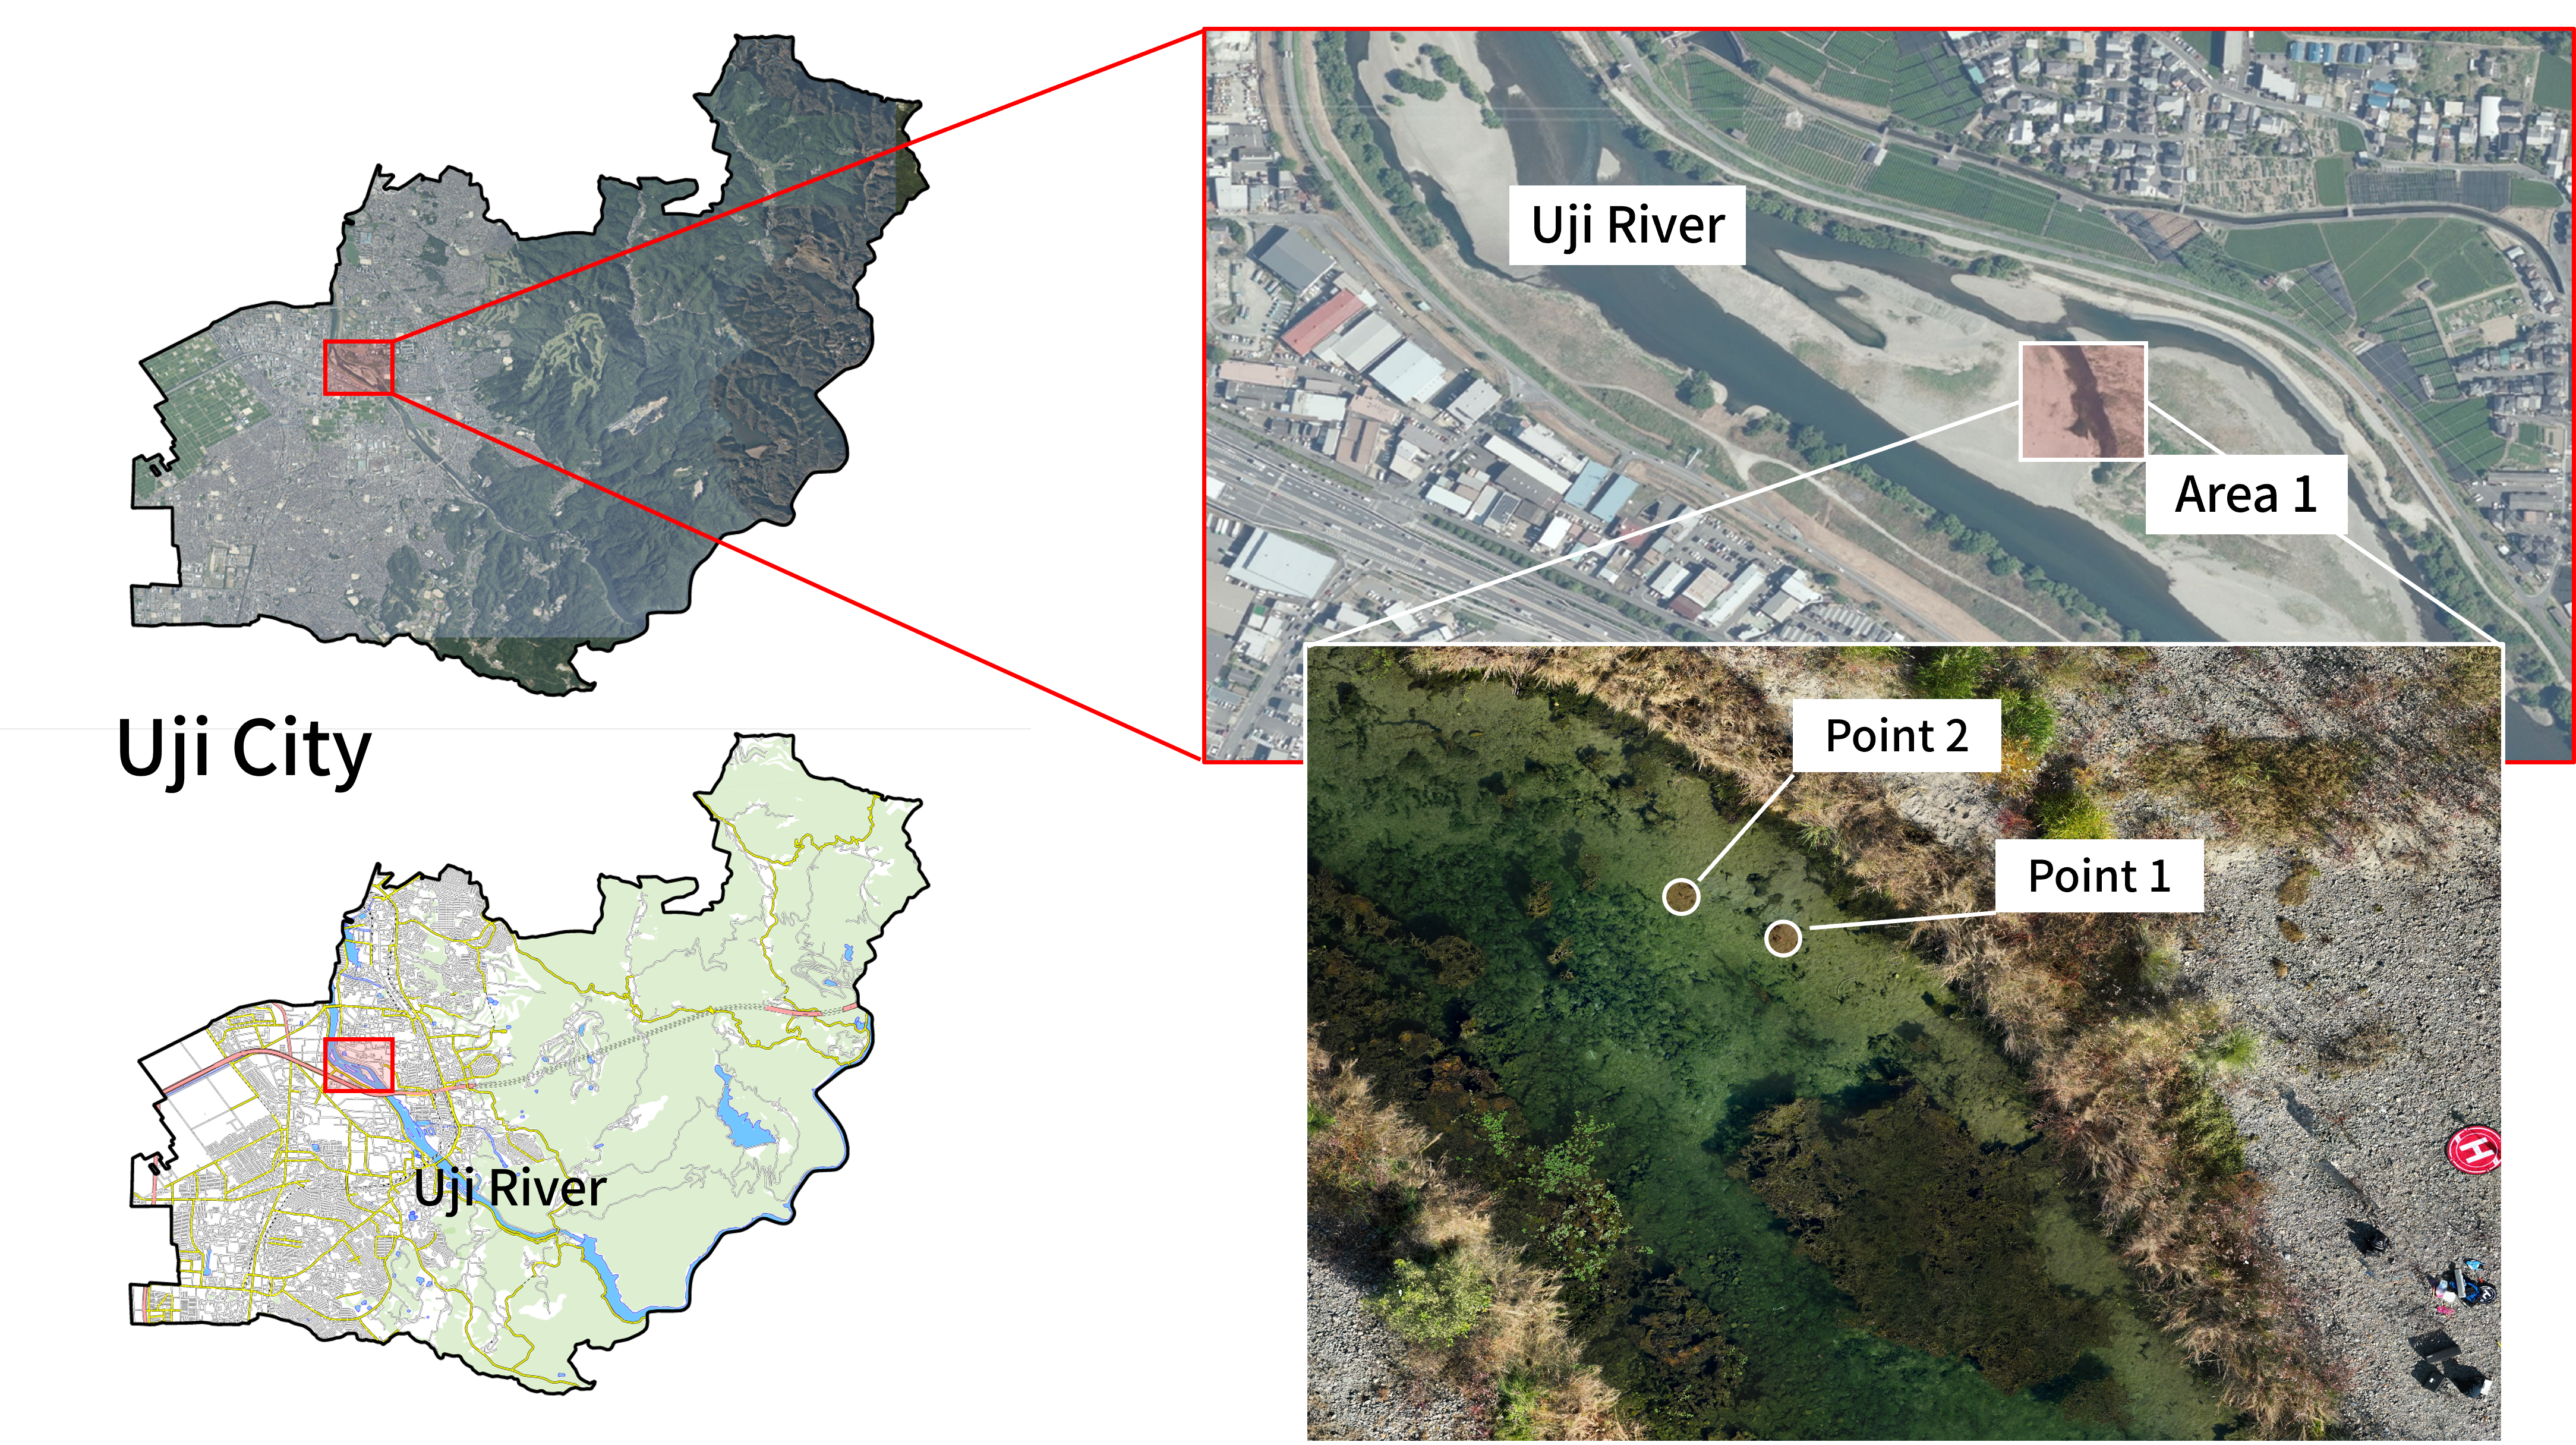
\includegraphics[height=10cm, keepaspectratio]{figure/60_data/area1.png}
    \caption{調査地域の概要。}
    \label{fig:area1_map}
  \end{subfigure}

  % 全体のキャプション
  \caption{
    調査対象地域の概要図。
    対象は、日本の京都府に位置する宇治市街を流れる宇治川の中流域である。
    本流から分派し水が滞留している箇所を対象にUAVから撮影を行った。
    広域航空写真は国土地理院~\cite{gsi_aerial_photo}、地図はOpen Street Map~\cite{OpenStreetMap}を使用した。
  }
  \label{fig:study-area}
\end{figure}

\missingfigure{scale Bar入れるの忘れてた!!}

\subsection{Study Area}\label{subsec:study-area}



% \begin{figure}[htbp]
%   \centering
%   \includegraphics[width=0.70\textwidth]{figure/60_data/study_area_overview.png}
%   \caption{調査対象地域の概要図。京都府宇治市の宇治川中流域でUAV調査を行った。}
%   \label{fig:study-area}
% \end{figure}

実世界における手法の検証には、京都府宇治市を流れる宇治川中流域にて取得したデータセット(Real-world data)を使用した。
データの取得は2025年11月15日の午前9:00から10:30にかけてArea1を対象に実施した
%(\cref{fig:study-area})
。
% データの取得は2025年11月15日の午前9:00から10:30にかけて実施し、同水域内の異なる2箇所(Area 1, Area 3)を対象とした。
\note{まだArea3を使用するか決めていない。2が環境が異なる(大きな礫が多い河床)だが、RTK情報がないため厳しい。3は試したいが、影とそれ以外の輝度差の大きい条件}
撮影時の気象条件は晴れであり、Area 1観測時における気温は12.8$^\circ$Cから16.3$^\circ$C、風速は0.5から0.9 m/sと極めて穏やかで、UAVおよび光学センサーによる水域観測に最適な環境であった。
% \url{https://www.data.jma.go.jp/stats/etrn/view/10min_s1.php?prec_no=61&block_no=47759&year=2025&month=11&day=15&view=}
本調査では、流速が速い本流ではなく、流れから分派し水が滞留している副次的な水路(Second channel)を対象とした。
この水域は波が穏やかで透明度が極めて高い。

% \subsubsection{Area 1}\label{subsec:area-1}
目視による推定最大水深は約1.5mであり、水面の一部には浮遊植物が確認された。
また、河床には藻類が生育しており、これにより水底が均質な砂礫ではなく視覚的に豊富なテクスチャを有している。
これは後述する画像からの三次元再構成を有利にする条件である。
取得されたUAV画像の特徴的な例は、%\cref{fig:field-data}%
に示す。

% \begin{figure}[htbp]
%   \centering
%   \includegraphics[width=0.70\textwidth]{figure/60_data/}
%   \caption{
%     各AreaのUAV画像の特徴的な例。
%     }
%     \label{fig:field-data}
% \end{figure}


% \note{
%   * ここでは、撮影エリアでの特徴に終始するぞ。
%   * 水面には水草が浮いているぞ。
%   * 本流ではなく、水たまりになっているSecond Channelにおいて撮影したぞ。
%   * 最大深度は1.5mほどだと推定されるぞ。
%   * Textureも比較的豊富だぞ。
%   * 透明度が高く、波も穏やかだぞ。
%   * 気温や湿度、天気はこの程度だった。(撮影時14度、湿度60\%、快晴)(後に正確に調べ直す)
% }


\subsection{UAV Platform}\label{subsec:uav-platform}


\begin{figure}[htbp]
  \centering

  \begin{minipage}[t]{0.45\linewidth}
    \centering
    \includegraphics[height=4cm, keepaspectratio]{figure/60_data/mavic3e.png}
    \caption{DJI Mavic 3 Enterprise}
    \label{fig:mavic3e}
  \end{minipage}
  % \hspace{0.5cm}
  \hfill
  \begin{minipage}[t]{0.45\linewidth}
    \centering
    \includegraphics[height=4cm, keepaspectratio]{figure/60_data/area1_riverbed-from-ground.JPG}
    \caption{地上から撮影したArea 1の河床。水面には浮遊植物、河床には藻類が生育している。}
    \label{fig:area1_riverbed-from-ground}
  \end{minipage}

  % \caption{#8}
  % \label{#9}
\end{figure}

画像の取得には、RTK-GPS(Real-Time Kinematic Global Positioning System)を搭載したUAV(Unmanned Aerial Vehicle)プラットフォームを使用した。
RTK測位を用いることで、センチメートル級の高精度な位置情報が各画像に付与されるため、地上基準点(GCP: Ground Control Points)を現地に設置することなく、高精度なSfM(Structure from Motion)処理が可能となっている。
\checkref{根拠となる論文を引っ張ってくる}

また、本研究では水底の三次元形状およびテクスチャを鮮明に捉えることを最優先としたため、カメラレンズに円偏光(Circular Polarized Light :CPL)フィルターを装着した。
これにより、水面における太陽光の反射(Sun Glint)を物理的に抑制している。
偏光フィルターの使用は取得画像の放射輝度値(Radiance)に影響を与え、厳密なラジオメトリック補正の不確実性を増加させる可能性があるが、本研究の範囲においては水面反射に伴う環境光のモデル化を考慮していないため、水面下の可視性を最大化するアプローチを採用した。


画像の取得には、RTK-GPS(Real-Time Kinematic Global Positioning System)を搭載した商用UAV、DJI Mavic 3 Enterprise\cite{DJI-Mavic-3-Enterprise}を使用した。
本機体は4/3型CMOSセンサー(有効画素数20MP)を搭載し、最大5280×3956ピクセルの高解像度画像を取得可能である
(\cref{tab:drone-spec}を参照)。
レンズは35mm判換算で24mm相当(FOV: 84$^\circ$、絞り: f/2.8-f/11)の広角レンズを使用している。
撮影時は、絞りをf/2.8に固定している。
\note{被写界深度を大きくやレンズ歪みを小さくするため、ピンホールカメラに近づけるよう小さな絞り(→f/11)を使用するべきだが、Motion Blurを抑制するためにシャッタースピードを高くすることが優先のため、デフォルトで多いな口径を使用しているのか。
DroneのObliqueを含めたPath設定・ シャッタースピードの固定、含めもっとたくさん設定できることが合った。
https://gemini.google.com/app/fc2bebc9e9d48912
}
RTK測位の精度は水平方向で1cm + 1ppm、垂直方向で1.5cm + 1ppm(RMS)であり、地上基準点(GCP: Ground Control Points)を現地に設置することなく、センチメートル級の絶対位置精度を持つSfMモデルの構築が可能である。
\checkref{根拠となる論文を引っ張ってくる}
% \note{ppmは「100万分の1」という意味です。測位においては、**「基準局から1km(100万mm)離れるごとに、1mmの誤差が加算される」**ことを意味します。 つまり、基準局と移動局(ドローンやトラクターなど)の距離(ベースライン)に比例して増える誤差です。}

また、本研究では水底の三次元形状およびテクスチャを鮮明に捉えることを最優先としたため、カメラレンズに円偏光(CPL)フィルターを装着した。
これにより、水面における太陽光の反射(Sun Glint)を物理的に抑制している。
偏光フィルターの使用は取得画像の放射輝度値(Radiance)に影響を与え、厳密なRadiometic Correction(\cref{sec:color-correction})の不確実性を増加させるが、
本研究の範囲においては水面反射における環境光による反射を考慮していないため、水面下の可視性を最大化するアプローチを採用した。


\begin{table}[htbp]
  \centering
  \caption{UAVプラットフォームおよびカメラの主要諸元}
  \label{tab:drone-spec}
  \begin{tabular}{@{}ll@{}}

    \toprule
    \textbf{Category} & \textbf{Specification} \\
    
    \midrule
    \textbf{UAV Platform} & \\
    \quad Model & DJI Mavic 3 Enterprise \\
    \quad Positioning System & Onboard RTK Module \\
    
    \midrule
    \textbf{Camera Specifications} & \\
    \quad Image Sensor & 4/3 CMOS \\
    \quad Effective Pixels & 20 MP \\
    \quad Max Image Size & 5280 $\times$ 3956 pixels \\
    \quad Field of View (FOV) & 84$^\circ$ \\
    \quad Equivalent Focal Length & 24 mm \\
    \quad Aperture & f/2.8  \\ % -- f/11 だが、撮影時はf/2.8で固定?
    \quad Focus Range & 1 m to $\infty$ \\
    \quad Additional Filter & Circular Polarizing (CPL) Filter \\
    
    \midrule
    \textbf{RTK Positioning Accuracy} & \\
    \quad Horizontal (RMS) & 1 cm + 1 ppm \\
    \quad Vertical (RMS) & 1.5 cm + 1 ppm \\

    \midrule
    \textbf{Flight Mission} & \\
    \quad Flight Altitude from Water Level & 12 m \\
    \quad Nadir Images & 108 \\
    \quad Overlap Rate & 90\% \\
    \quad Side Overlap Rate & 90\% \\
    \quad Oblique Images & 80 \\
    \quad Tilt Angle & 45$^\circ$ \\

    \bottomrule
  \end{tabular}
\end{table}

\subsection{Data Acquisition}\label{subsec:data-acquisition}

\begin{table}[htbp]
  \centering
  \caption{撮影条件の詳細}
  \label{tab:flight-mission}
  \begin{tabular}{@{}ll@{}}

    \toprule
    \textbf{Flight Mission} & \\
    \midrule
    \quad Flight Altitude from Water Level & 12 m \\
    \quad \# of Nadir Images & 108 \\
    \quad Overlap Rate & 90\% \\
    \quad Side Overlap Rate & 90\% \\
    \quad \# of Oblique Images & 80 \\
    \quad Oblique Angle & 30$^\circ$ $sim$ 45$^\circ$ \\

    \bottomrule
  \end{tabular}
\end{table}

UAVによる撮影は、多視点性を確保し、画像からの三次元再構成の幾何的な推定を強めるため、直下視(Nadir)および斜め視(Oblique)の二種類のカメラアングルを組み合わせて実施した。
高度は地上高(AGL: Above Ground Level)12mという低高度で実施し、高空間分解能の画像を確保した。
ただし、後述するワークフロー(\cref{sec:workflow})ではSfM処理は最大解像度で行ったが、提案手法のRefractive-Aware Gaussian Splattingは1/4にダウンサンプリングした画像を用いた。

Nadir画像は、オーバーラップ率を90\%、サイドラップ率を90\%に設定し、自動航行により108枚取得した。
\note{OL,SL を覚えていない。リモコンから確認しないと。計算によるとだいたい90\%になる。85\%撮った気もする}

Oblique画像については、特定の一点を中心とするマニュアル操作により、カメラのオフナディア角を主に約30$^\circ$ $sim$ 45$^\circ$ (一部、60$^\circ$を含む)で、円軌道を描くように対象地点を見下ろしながら、80枚を取得した。
カメラの角度および飛行経路の詳細は、%\cref{fig:camera-path}
に定性的に示す。

\IncludeTwoImages[6cm]
{figure/60_data/area1-4_0001.JPG}
  {Nadir画像の例}
{figure/60_data/area1-6_0059.JPG}
  {Oblique画像の例}
{Area1におけるUAV画像の例}
{fig:area1}

\begin{figure}[htbp]
  \centering
  \includegraphics[width=0.80\textwidth]{figure/60_data/camera-path.png}
  \caption{
    Area1におけるカメラパスと姿勢。NadirとObliqueの2種類のカメラアングルを組み合わせて撮影した。
    }
    \label{fig:camera-path}
\end{figure}


また、推定された水深精度の定量的な評価を行うため、現地調査において水深データの取得を行った。
調査者が実際に水域に入り、代表的なポイントに検証用ターゲットを設置した上で(\cref{fig:area1_map}参照)、メジャーを用いた手動計測により水深を測定した。
測定された検証点の水深は、それぞれ61cmおよび71cmの計2点である。
地点の正確な座標は水域内であるため計測できず、検証時には、三次元復元データからターゲットを視認し、手動で座標を特定した。

\begin{figure}[htbp]
  \centering

  \begin{minipage}[t]{0.45\linewidth}
    \centering
    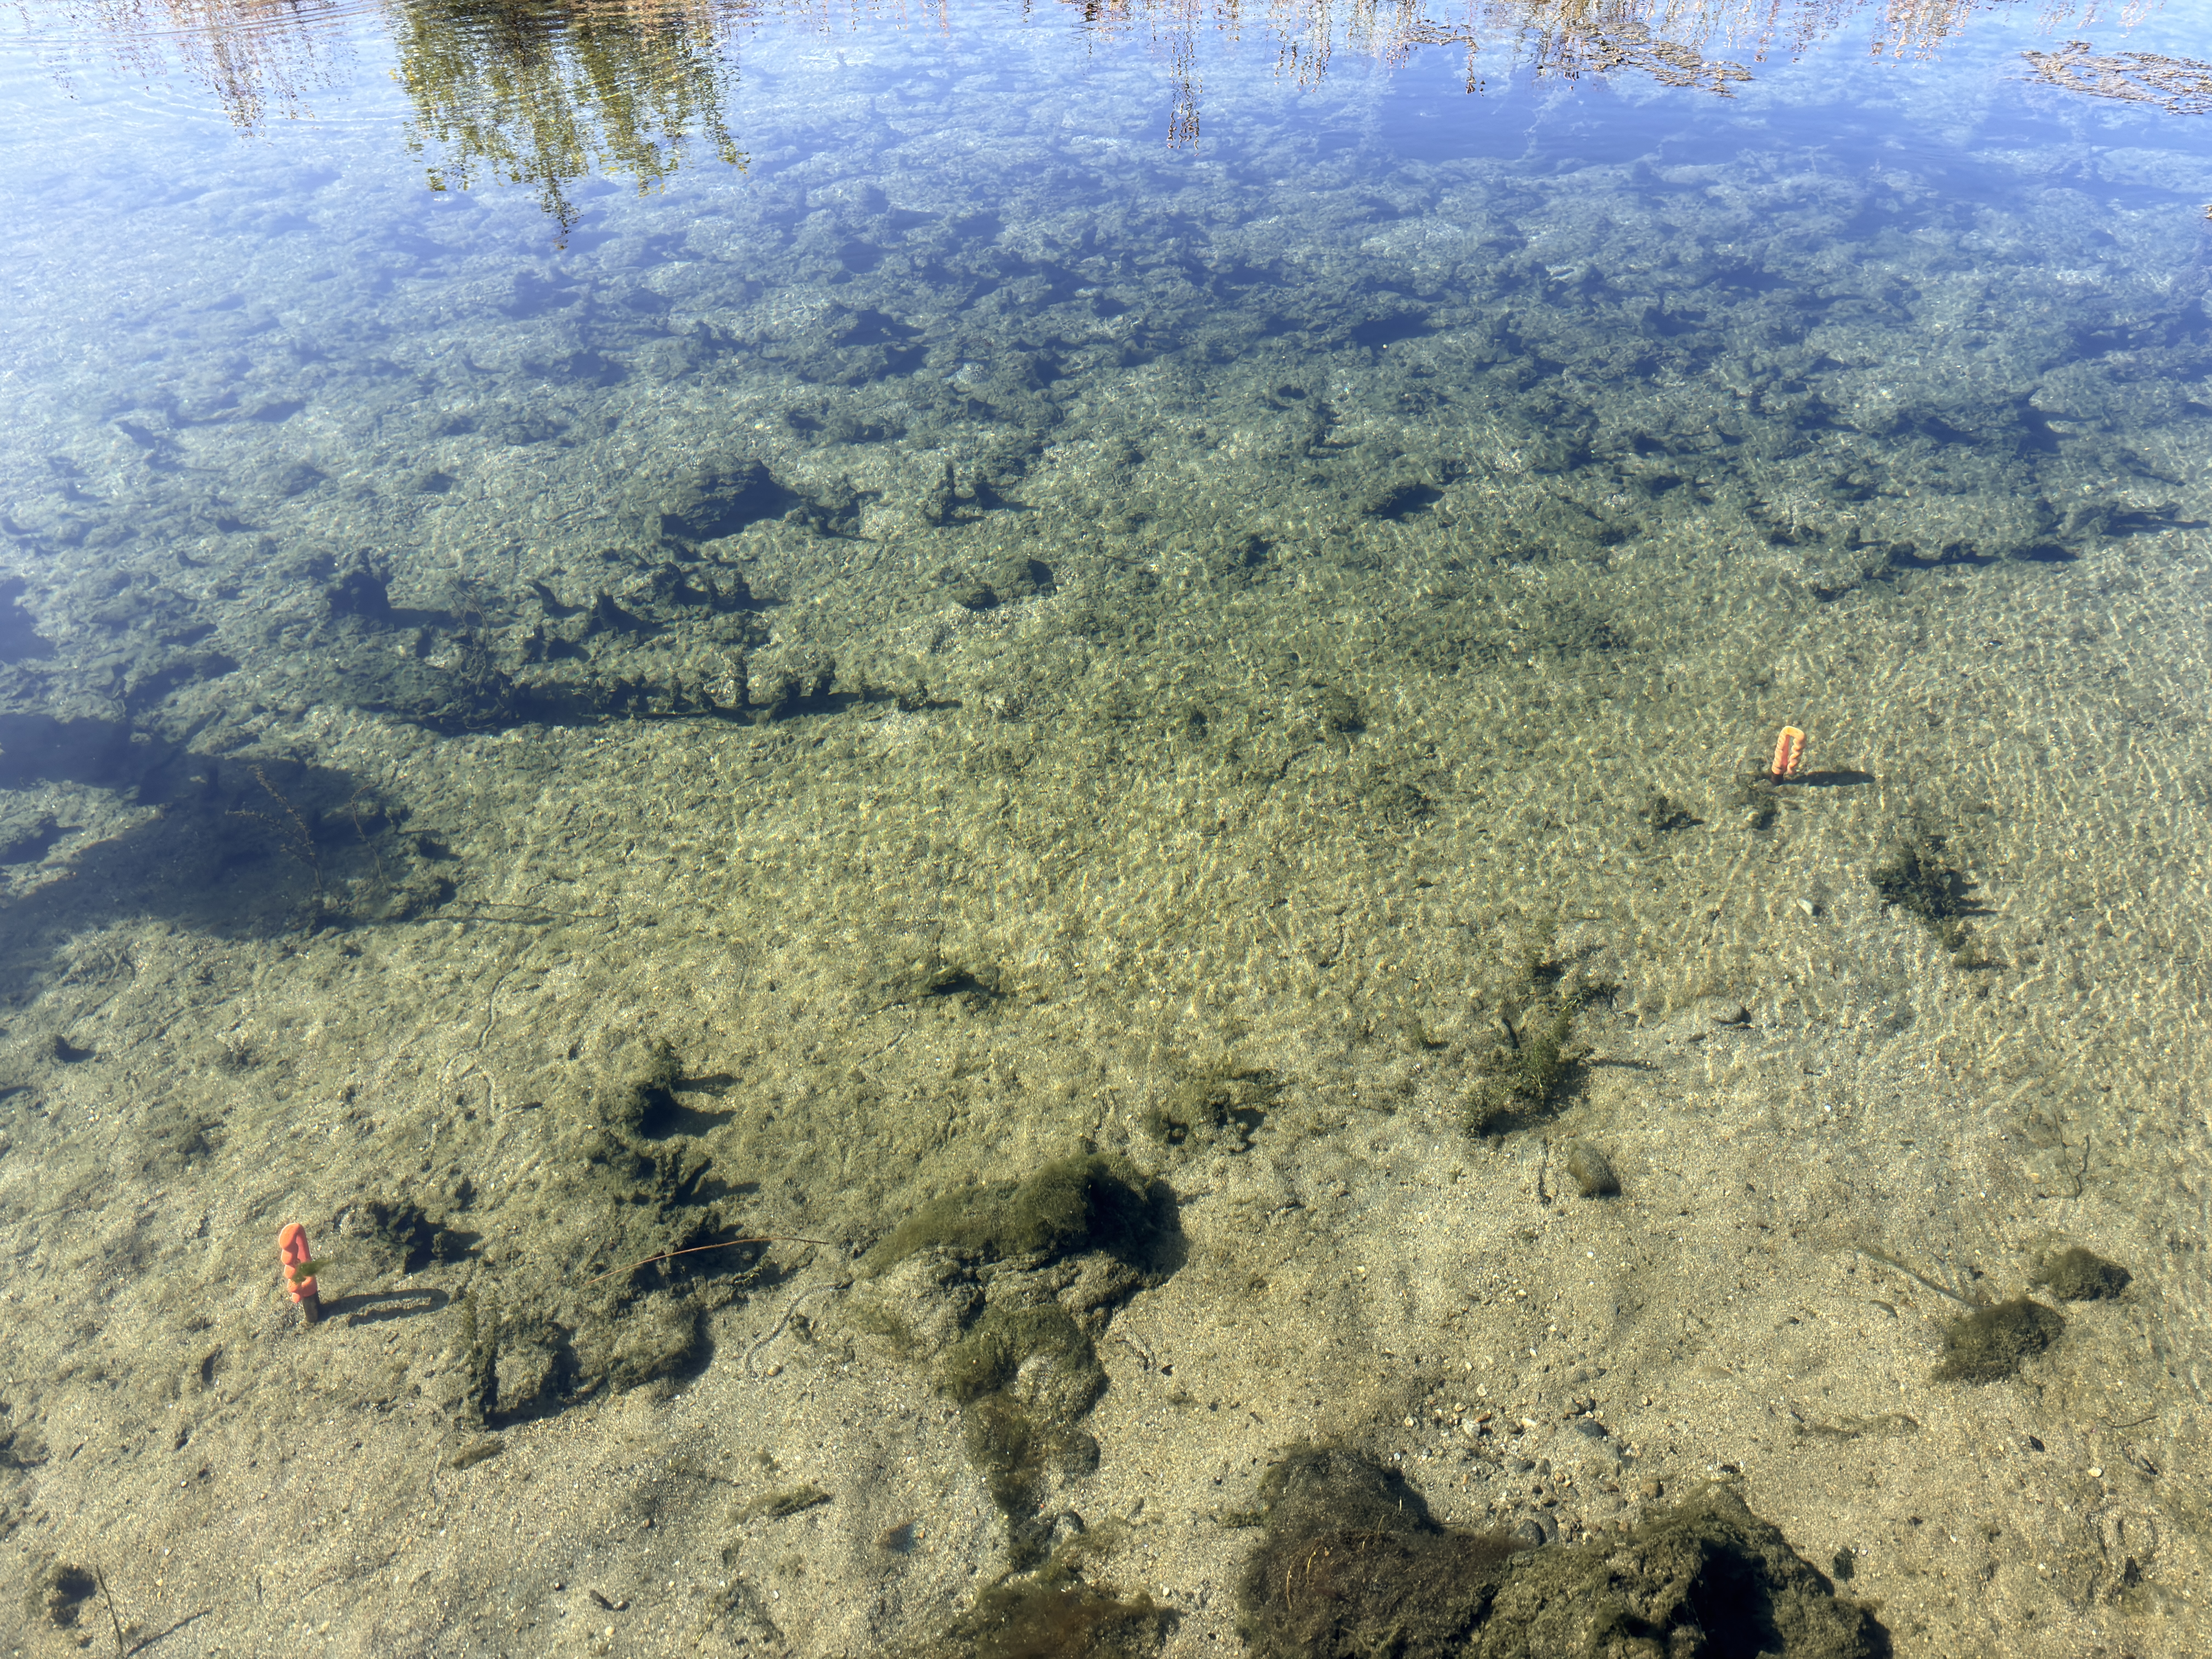
\includegraphics[height=8cm, keepaspectratio]{figure/60_data/area1_riverbed-and-mark.JPG}
    \caption{Area1における検証ターゲットの設置例}
    \label{fig:area1_mark}
  \end{minipage}
  % \hspace{0.5cm}
  \hfill
  \begin{minipage}[t]{0.45\linewidth}
    \centering
    \includegraphics[height=8cm, keepaspectratio]{figure/60_data/area1_mark_measure.jpg}
    \caption{検証ターゲットの測定方法}
    \label{fig:area1_mark_measure}
  \end{minipage}

  % \begin{minipage}[t]{0.45\linewidth}
  %   \centering
  %   \includegraphics[height=5cm, keepaspectratio]{figure/60_data/area1_mark_measure.jpg}
  %   \caption{Area1における検証ターゲット(Point1, Point2)の地点}
  %   \label{fig:area1_mark_measure}
  % \end{minipage}

  % \caption{#8}
  % \label{#9}
\end{figure}

\note{
  Future Work
  撮影時のシャッタースピードは固定できておらず、シャッタースピードに応じたガンマ補正を考慮した輝度値補正を行うべき。
}


% \note{
%   * 偏光レンズを用いたぞ。(これはPlatformに入れるべき話かもしれぬ。)cite(Joyce2018Drone-marine-surveyand_how-to)で、偏光レンズの言及あり(ただし曇りの日)
%   Radiometic Correctionに影響を与えるかもしれないが、どのみち環境光の水面での反射は考慮できていないから、撮影時の河床を鮮明に撮像できることを優先した。
%   * Nadirとオブリークで撮影したぞ。https://gemini.google.com/app/42efe917f2e9b646
%   * 検証点を自分で中に入り、設置し、手動で深度を測定したぞ。それぞれの深度は図のように61cm70cmだったぞ。
%   * 後のWorkflowで解説するが、cite(Joyce2018Drone-marine-surveyandhow-to)によると、水中でのGCP設置は困難であり、SfMによるカメラキャリブレーションの正確性を担保するため、地上を画像内に移せるようにする。
% }

% \note{
%   シャッタースピードが固定されておらず、
%   DJI20251115092203-0002_V.JPG では、1/250で画像が明るくいい感じなのに、
%   DJI20251115092309-0078_V.JPG では、1/640で画像がかなり全体的に暗くなっている。
%   ISPRS前に補正できないか。良くない。
%   https://gemini.google.com/app/42efe917f2e9b646
% }

%!TEX root = ../main.tex
\chapter{Experiments}\label{chap:experiments}
\section{Workflow}\label{sec:workflow}

本節では、実環境データを対象にした、屈折を考慮した水中3次元再構成のための完全なパイプラインを概説する。

\begin{figure}[htbp]
  \centering
  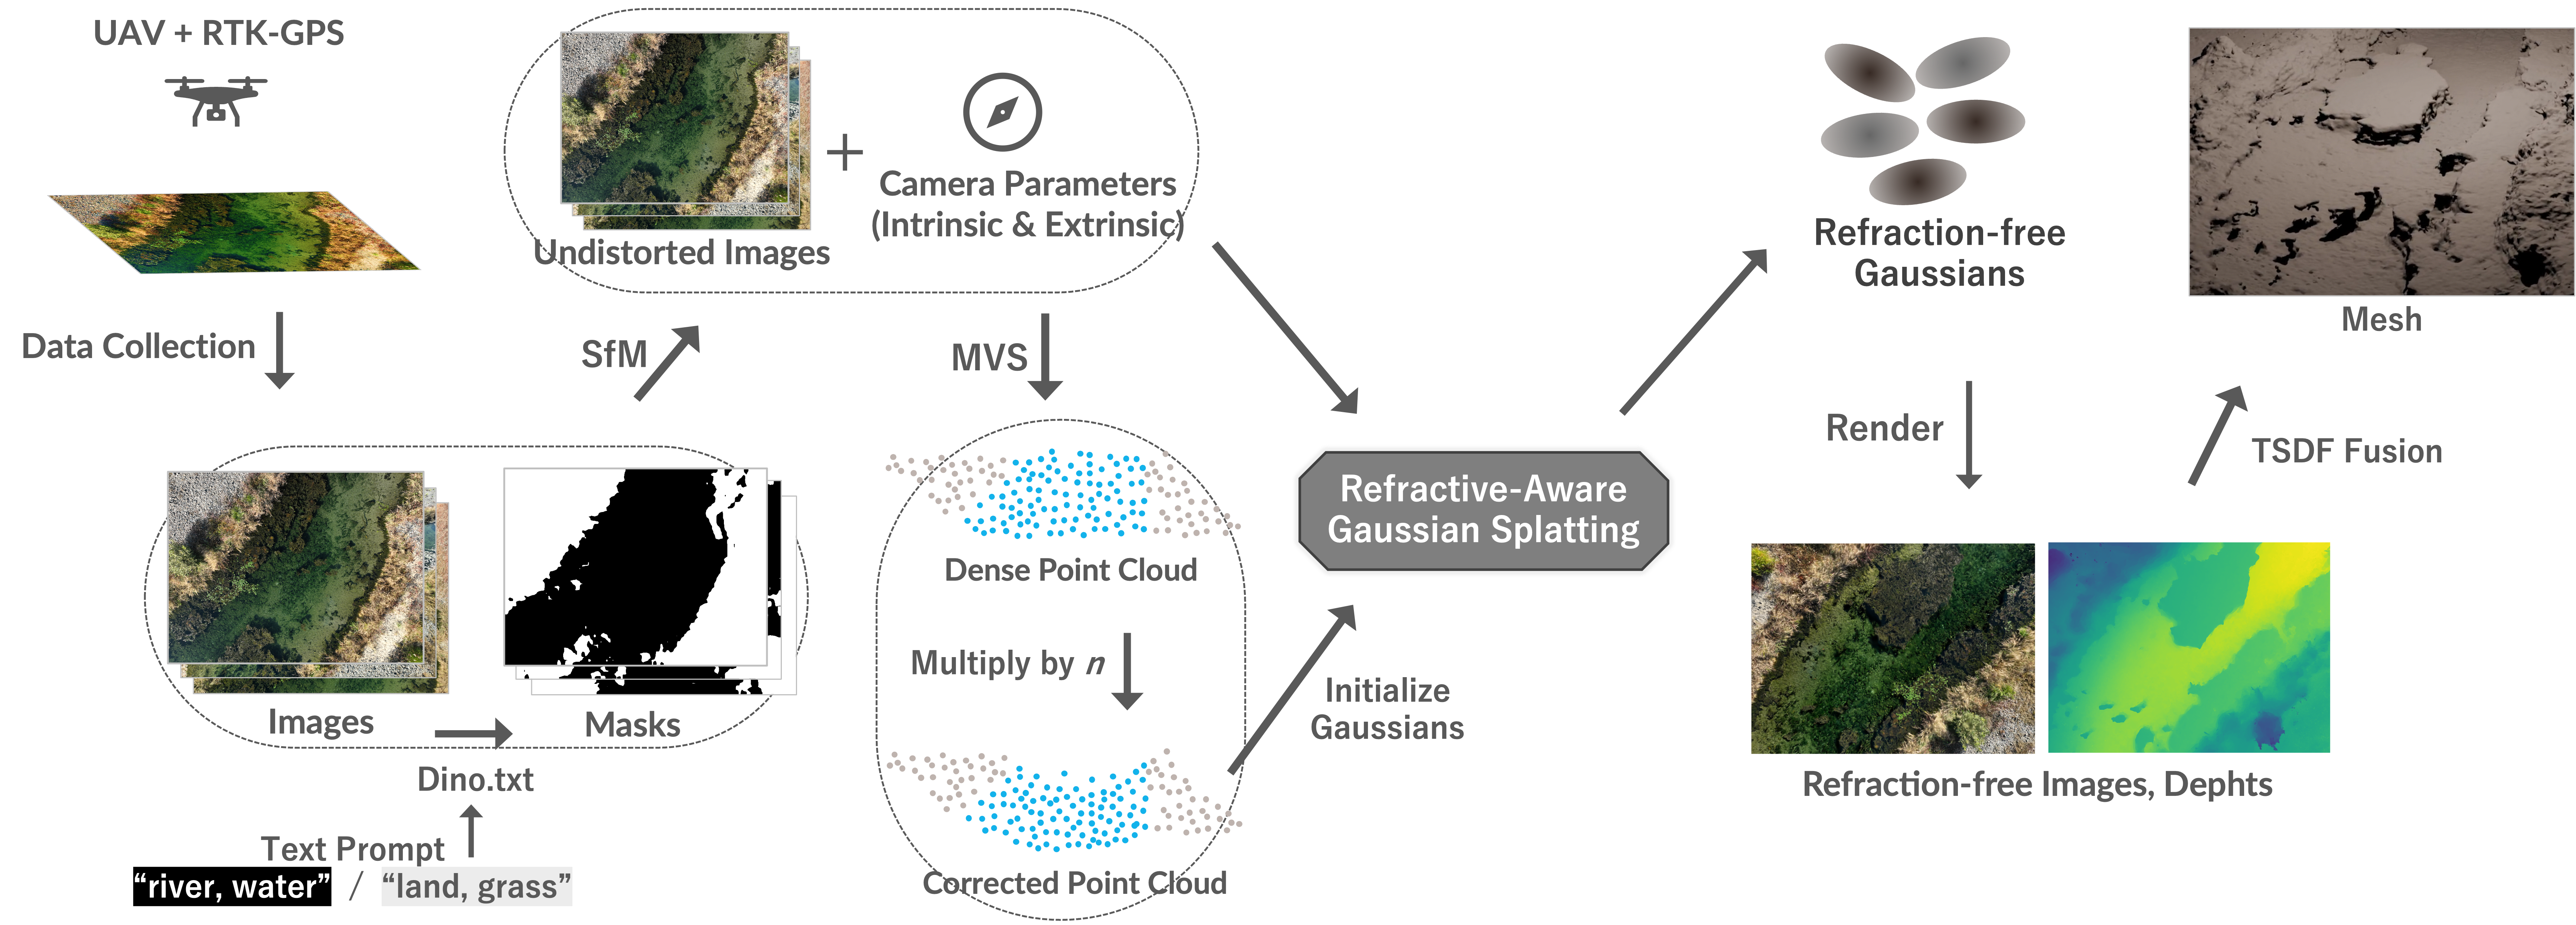
\includegraphics[width=0.95\textwidth]{figure/70_experim/workflow.png}
  \caption{
    実環境データを対象にした、屈折を考慮した水中3次元再構成のための完全なパイプライン。
    }
    \label{fig:workflow}
\end{figure}


\subsection{データ収集とセマンティック・セグメンテーション}\label{subsec:data-acquisition}

\subsubsection{UAVによる画像取得とジオリファレンス}

RTK-GPS(Real-Time Kinematic GPS)を搭載したUAVを用いて、河川および陸地を含む対象領域を撮影する。
各画像には、RTK測位による高精度なカメラ外部パラメータ(緯度・経度・高度)がメタデータとして付与される。
これにより、SfMにおいての拘束条件を追加し、実スケールでの再構成精度を保証する。
\note{Field Studyの具体的な詳細は前章ののDatasetで}

\subsubsection{Vision-Language Modelによるマスク生成}

RA-GSは、入力として正確なカメラ内部・外部パラメータを期待する。
これらは既存のパイプラインと同様\cite{Kerbl2023ToG_3DGS,Schonberger2016ECCV_PatchMatchStereo}に、SfMを用いて推定する。
屈折面が存在することで、SfM前提の光の直進性が成立しなくなり、精度は悪化し、また、屈折の影響の大きいシーンでは特徴点のRANSACによる整合ができなくなる場合も考えれる。
そこで、SfMに入力画像とその除外エリアを示すマスク画像を入力する。
これは、一般のシーンの三次元復元でも一般的な手法であり、陸域であれば、人物や車両などの移動体、鏡などの反射物を除外する。
本研究での結果は商用フォトグラメトリソフトであるRealityScan\cite{RealityScan}を使用したが、COLMAPや他のフォトグラメトリソフトウェアでも同様の手法が実現可能である。

この手法では、画像の取得で常に十分な陸域を含める必要があり、UAVの高度や角度に関しての柔軟性を失う。
後述するように、RA-GSでは、カメラ外部パラメータに関しての勾配も追跡可能で、Photometricな情報からのカメラポーズ推定も可能である。
外部パラメータの初期値にはGPSによるジオリファレンスとドローンのログデータによる姿勢方角情報を使用する。
現在は内部パラメータまでの最適化はできないため、予めカメラはキャリブレーションを行い、歪み補正を行っておく。
また、R-SfM\cite{Makris2024_refractive-aware-sfm}を用いて、屈折領域込みでのカメラポーズ推定も可能である。
\note{現在Codeも公開されているが、正直いい実装には思えなかった。}


\begin{figure}[htbp]
  \centering
  \includegraphics[width=0.95\textwidth]{figure/70_experim/DinoTXT.png}
  \caption{
    Dino.txtの概要。
    \cite{Jose2025CVPR_DINOv2-Text}から引用。
    (左):DinoV2\cite{Oquab2023_DINOv2}による自己教師あり学習(Self-Supervised Learning: SSL)による特徴量をPCAで可視化したものである。
     (本研究では、DinoV3\cite{Simeoni2025_DINOv3}を使用している)
    (中央):は学習済SSLと、ゼロから学習したテキストエンコーダを整合させるトレーニング戦略を示す。
    視覚エンコーダ上に軽量なビジョンブロックを追加することで、テキストとの整合性をさらに向上させている。
    モデル全体はわずか5万イテレーションで学習可能であり、ゼロショット分類およびオープン語彙セグメンテーションの両タスクにおいて最先端性能を達成した(右):出力結果例。(入力画像と、それに対応する zero-shot 分類や open-vocabulary セグメンテーションの結果)。
    }
    \label{fig:DinoTXT}
\end{figure}

\missingfigure{実際のマスク作成例。定量も含めて示す}

本研究の浅水域を対象とした、水域と陸域を区別する。
前章で示した宇治川のデータを例に上げると、水面はマスクにより除外し(0値)、陸域には陸地や草木などが含まれ、それらを非マスクとして残す(1値)。
今回は非マスクとして扱ったが、風の強い日では草木は揺らめくことで幾何推定の精度が悪化するため、その場合はマスクとして除外する必要があるし、
宇治川データセットでは水面に多数の浮草が凝集して存在し、それらは屈折の影響を受けないため、SfMによる幾何推定の対象に含めたいため非マスクとして抽出したい。
このように、
Automated: Manual labeling for hundreds images is time consuming ! 
Robustness:  robustly across diverse environments.
Zero-Shot:  Fine-tuning models for each new environment is also time consuming impractical !
Controllability : flexible specification using natural language.“I want to remove those ‘ship and shadow’ ! ”
のような条件が必要。



\note{
  Automated: Manual labeling for hundreds images is time consuming ! 
  Robustness:  robustly across diverse environments.
  Zero-Shot:  Fine-tuning models for each new environment is also time consuming impractical !
  Controllability : flexible specification using natural language.“I want to remove those ‘ship and shadow’ ! ”
}

本研究では、オープン語彙物体検出モデル(DINO.txt\cite{Jose2025CVPR_DINOv2-Text,Simeoni2025_DINOv3})を採用し、テキストプロンプトによるゼロショット・セグメンテーションを行う。
\note{Dinoの説明は、40prelimのForward 3D Reconstructionでシたいと思ったがしないかも}
具体的には、"river, water" および "land, grass" というテキストプロンプトからノイズを除去した二値マスク(Binary Masks)を生成する。




% \subsubsection{SfMによる疎な再構成}

% まず、特徴点抽出(SIFT \parencite{Lowe2004_SIFT}等)とマッチングを行い、インクリメンタルなSfM(Structure from Motion)パイプライン(例:COLMAP \parencite{Schonberger2016ECCV_PatchMatchStereo})を適用する。
% ここでは、レンズの放射歪みおよび接線歪みを考慮したカメラモデルを用いて内部パラメータを推定すると同時に、全画像の6自由度(6-DoF)のポーズを推定する。
% 出力として、歪み補正済み画像(Undistorted Images)とカメラパラメータが得られる。

% \subsubsection{MVSによる密な点群生成}

% 推定されたカメラパラメータに基づき、MVS(Multi-View Stereo)アルゴリズム(例:PatchMatch Stereo \parencite{Bleyer2011BMVC_PatchMatchStereo})を適用し、画素ごとの深度マップを推定する。
% 複数の深度マップを幾何学的整合性(Geometric Consistency)チェックに基づいて統合することで、シーン全体の密な点群(Dense Point Cloud)を生成する。

% \subsection{スネルの法則に基づく点群の初期化}\label{subsec:physics-initialization}

% MVSで生成された点群のうち、水面下に位置する点は、水と空気の境界での光の屈折を無視した「見かけの深度(Apparent Depth)」として計算されている。
% これをそのままGaussian Splattingの初期値として用いると、最適化が局所解に陥るリスクがあるため、物理的な補正を行う。

% \subsubsection{深度スケーリングによる補正}

% セマンティック・マスクにより「水域」と判定された領域に対応する点群に対し、水の屈折率 $n$(淡水を想定し $n \approx 1.33$)を用いた深度補正を行う。
% 近軸近似(Paraxial Approximation)の仮定下において、実深度 $d_{\mathrm{real}}$ と見かけの深度 $d_{\mathrm{apparent}}$ の関係は以下のように表される:
% \begin{equation}\label{eq:paraxial-depth-correction}
%   d_{\mathrm{real}} \approx n \cdot d_{\mathrm{apparent}}
% \end{equation}
% 本手法では、水域の点群の深度値に対して一律に係数 $n$ を乗じる操作を行うことで、点群を幾何学的に正しい位置へと簡易的に移動させる。
% これにより得られた「補正済み点群(Corrected Point Cloud)」は、後続のRefractive-Aware Gaussian Splattingに対し、物理的に妥当な初期分布(Warm Start)を提供する役割を果たす。

% \subsection{Refractive-Aware Gaussian Splattingによる最適化}\label{subsec:refractive-gs}

% 補正済み点群を入力とし、屈折モデルを組み込んだレンダリングパイプラインを通じて3次元ガウシアンのパラメータを最適化する。
% 詳細は\cref{chap:method}の手法説明に譲る。

% \subsection{ボリューメトリック融合によるメッシュ再構成}\label{subsec:mesh-reconstruction}

% 最適化されたガウシアン表現は、離散的な点群(Splat)の集合であるため、地形解析等に適した連続的な表面モデルを得るための後処理を行う。

% \subsubsection{TSDF Fusion}

% 学習済みのガウシアンからレンダリングされた高精度な深度マップおよび法線情報を入力とし、TSDF(Truncated Signed Distance Function)Fusion \checkref{Curless and Levoy (1996) SIGGRAPHのTSDF論文を引用}を行う。
% 対象空間をボクセルグリッドに分割し、各ボクセルに表面までの符号付き距離を格納して統合することで、観測ノイズを平滑化する。

% \subsubsection{Marching Cubes法によるメッシュ化}

% 蓄積されたTSDFボリュームに対し、Marching Cubesアルゴリズム \checkref{Lorensen and Cline (1987) SIGGRAPHのMarching Cubes論文を引用}を適用して等値面(Iso-surface)を抽出する。
% これにより、水底の岩や地形の起伏を含む、幾何学的位相の整った三角形メッシュ(Mesh)が出力される。
% このメッシュは、従来のフォトグラメトリ手法では困難であった、屈折の影響を排除した真の水底形状を表している。

% 実装はOpen3Dは使用した\cite{Open3D}。

% \input{sections/70_experim_implementation.tex}



% --- 謝辞 ---
\input{sections/90_acknowledg.tex}

% --- Appendix ---
%!TEX root = ../main.tex
\chapter{APPENDIX}

\section{見かけの深度 (Apparent Depth) の導出}\label{sec:apendix-apparent-depth}

カメラ座標系においてカメラ位置を$z$軸上$\left(0, 0, H\right)$に、また水面を平坦な$xy$平面(法線ベクトルが一定、すなわち静水面とする)に配置する。
水中に存在する各3次元Gaussianプリミティブの位置$\bm{p}$は$\left(x, y, z\right)$(ただし$z<0$)で表される。
簡単化のため、問題を2次元化し、位置を$r = \sqrt{x^2 + y^2}$として$rz$-平面上に射影する(\cref{fig:rz}を参照)。

幾何光学原理およびスネルの法則(Snell's law)より、水中点$\bm{p}$を観測するカメラ視点から見た「見かけの位置」は、観測方向に依存せず定まる\cite{nassar1994_ApparentDepth,Missailidis2025_apparentDepth-leading}。
ここではその詳細な導出を示す。

Gaussian中心の見かけの位置を$\bm{p}'(r', z')$とする。
カメラ位置と見かけの位置$\bm{p}'$を結ぶ入射線と水面との交点を$(s, 0)$($0 < s < r$)とおく。

スネルの法則(空気屈折率$1$、水屈折率$n$、入射角$\theta_i$、屈折角$\theta_r$)は次式で表される。
\begin{equation}
  \sin \theta_i = n \sin \theta_r
\end{equation}

各三角関数項は、カメラ、交点、原点などで構成される三角形$\triangle OAI$, $\triangle IPC$により幾何的に表現できる。

上記関係から、$s$に関する四次方程式が導かれる。
\begin{equation}
\begin{split}
  (1-n^2)s^4 &+ 2(n^2-1)rs^3 \\
  &+ ((1-n^2)r^2 - n^2H^2 + z^2)s^2 \\
  &+ 2n^2H^2rs - n^2H^2r^2 = 0
\end{split}
\end{equation}
(実装ではニュートン法等で数値的に解く。)

わずかなずれ$\Delta s$を仮定し、$s+\Delta s$の交点、および$\theta_r+\Delta \theta_r$の微小変化を考える。三角形$\triangle IP'C'$の関係より、
\begin{equation}\label{eq:triangle-IP'C'}
  -z' \tan \theta_i  = r' - s 
\end{equation}
また、$\triangle I'P'C'$より
\begin{align}\label{eq:triangle-I'P'C'}
  -z' \tan \left(\theta_i + \Delta \theta_i \right) & = (r' - s) + (- \Delta s) \notag \\
  -z' \left( \sin \theta_i + \Delta \theta_i \cos \theta_i  \right) & = (r' -s - \Delta s) \left( \cos \theta_i - \Delta \theta_i \sin \theta_i \right) 
\end{align}

\cref{eq:triangle-IP'C'}と\cref{eq:triangle-I'P'C'}から$z'$を消去し、$\Delta \to 0$の極限をとると
\begin{equation}\label{eq:limit-r'}
  r' = s - \sin \theta_i \cos \theta_i \frac{d s}{d \theta_i}
\end{equation}
が得られる。

また、\cref{eq:triangle-IP'C'}と上式より
\begin{equation}\label{eq:z'_ds/dtheta_i}
  z' = \frac{d s}{d \theta_i} {\cos \theta_i}^2
\end{equation}

さらに、三角形$\triangle IPC$から
\begin{equation}\label{eq:r-s}
  r - s = - z \tan \theta_r
\end{equation}

これを$\theta_r$で微分すると
\begin{equation}\label{eq:ds/dtheta_r}
  \frac{d s}{d \theta_r} = z \cdot \frac{1}{{\cos \theta_r}^2}
\end{equation}

また、スネルの法則\eqref{eq:snell}を$\theta_i$で微分すると
\begin{equation}\label{eq:dtheta_r/dtheta_i}
  \frac{d \theta_r}{d \theta_i} = \frac{1}{n} \cdot \frac{\cos \theta_i}{\cos \theta_r}
\end{equation}

\eqref{eq:dtheta_r/dtheta_i},\eqref{eq:ds/dtheta_r}より
\begin{equation}\label{eq:ds/dtheta_i}
  \frac{d s}{d \theta_i} = \frac{z}{n} \cdot \frac{\cos \theta_i}{{\cos \theta_r}^3}
\end{equation}

以上をまとめると、見かけの位置$(r', z')$はそれぞれ
\begin{equation}
  \begin{split}
    (1-n^2)s^4 &+ 2(n^2-1)rs^3 \\
    &+ ((1-n^2)r^2 - n^2H^2 + z^2)s^2 \\
    &+ 2n^2H^2rs - n^2H^2r^2 = 0
  \end{split}
\end{equation}
と表される。


% --- 参考文献リスト出力 ---
\newpage
\addtocontents{toc}{\vspace{2em}}
\addcontentsline{toc}{section}{参考文献}

% --- Bibliography ---
\printbibliography[title={参考文献}]


% --- End of document ---
\end{document}

